\documentclass[lettersize,journal]{IEEEtran}
\usepackage{amsmath,amsfonts}
\usepackage{algorithmic}
\usepackage{algorithm}
\usepackage{array}
\usepackage[caption=false,font=normalsize,labelfont=sf,textfont=sf]{subfig}
\usepackage{textcomp}
\usepackage{stfloats}
\usepackage{url}
\usepackage{verbatim}
\usepackage{graphicx}
\usepackage{cite}
\hyphenation{op-tical net-works semi-conduc-tor IEEE-Xplore}
\usepackage{balance}
\usepackage{lipsum}
\usepackage{cuted}
\usepackage{units}
\usepackage{nicefrac, xfrac}
\usepackage[ngerman,english]{babel}
\usepackage{breqn}
\usepackage{autobreak}
\usepackage{tabularx}
\usepackage{indentfirst}
\usepackage{cases}
\usepackage{amssymb}
\usepackage{hyperref}
\usepackage[capitalise]{cleveref}
\usepackage[numbers,sort&compress]{natbib}
\usepackage{annotate-equations}
%\usepackage{mathtools, nccmath}
\usepackage{anyfontsize}
\setlength{\textfloatsep}{2.25pt}
\setlength{\abovecaptionskip}{-0.15cm}
\setlength{\belowcaptionskip}{-2cm}
\usepackage{nomencl}

\makenomenclature
\usepackage{etoolbox}
\renewcommand\nomgroup[1]{%
  \item[\bfseries
  \ifstrequal{#1}{I}{Index and set}{%
  \ifstrequal{#1}{P}{Parameters}{%
  \ifstrequal{#1}{V}{Variables}{}}}%
]}

\newcommand{\Rmnum}[1]{\uppercase\expandafter{\romannumeral #1}}
\newcommand{\slfrac}[2]{\left.#1\middle/#2\right.}
%\usepackage[nodisplayskipstretch]{setspace}
\allowdisplaybreaks
\tolerance=1000
\emergencystretch=5pt
\hyphenpenalty=5000
\exhyphenpenalty=100
\hyphenation{hy-phen-a-tion}
\def\code#1{\texttt{#1}}

\renewcommand{\tabularxcolumn}[1]{m{#1}}
\newcolumntype{L}{>{\RaggedRight\arraybackslash}X}
\newcolumntype{C}[1]{>{\Centering\arraybackslash%
        \hsize=#1\hsize\linewidth=\hsize}X}

\newenvironment{newsequation}{\small\begin{equation}}{\end{equation}}
\newenvironment{newsubequations}{\small\begin{subequations}}{\end{subequations}}

% \AtBeginDocument{%
%   \addtolength\abovedisplayskip{-0.5\baselineskip}%
%   \addtolength\belowdisplayskip{-0.5\baselineskip}%
% %  \addtolength\abovedisplayshortskip{-0.5\baselineskip}%
% %  \addtolength\belowdisplayshortskip{-0.5\baselineskip}%
% }

\hyphenation{ve-ry-lon-g-w-ord  ev-en-long-er-com-pound-word-with-no-spaces}
% \hyphenation{Duisauteiruredolorinre-prehenderitinvoluptatevelitesse-cillum doloreeufugiatnullapariatur}

\hyphenation{op-tical net-works semi-conduc-tor IEEE-Xplore}
\def\BibTeX{{\rm B\kern-.05em{\sc i\kern-.025em b}\kern-.08em
    T\kern-.1667em\lower.7ex\hbox{E}\kern-.125emX}}
\usepackage{balance}
\begin{document}
\vspace{-2.5in}
\title{ \vspace{-0.5em}
	{\fontfamily{stix}\selectfont
		\fontsize{24}{20}\selectfont
		Harnessing Bayesian Filter for Addressing Uncertain Variability in Chance-Constrained FDUC
	}
}
\vspace{-2.5in}
\author{\fontsize{11}{8} \selectfont Yiping Yuan, \textit{Member, IEEE}, Zhou Liu, \textit{Senior Member, IEEE}, Weihao Hu, \textit{Senior Member, IEEE},   Yuming Zhao, \textit{Member, IEEE}, Marjan Popov, \textit{Fellow, IEEE}, Qi Huang,
	\textit{Fellow, IEEE}, Zhe Chen, \textit{Fellow, IEEE} \vspace{-2.5em}}
%\thanks{Manuscript created October, 2020; This work was developed by the IEEE Publication Technology Department. This work is distributed under the \LaTeX \ Project Public License (LPPL) ( http://www.latex-project.org/ ) version 1.3. A copy of the LPPL, version 1.3, is included in the base \LaTeX \ documentation of all distributions of \LaTeX \ released 2003/12/01 or later. The opinions expressed here are entirely that of the author. No warranty is expressed or implied. User assumes all risk.}}

\markboth{Journal of \LaTeX\ Class Files,~Vol.~18, No.~9, September~2020}%
{How to Use the IEEEtran \LaTeX \ Templates}

\maketitle
\vspace{-2.5em}
\begin{abstract}
	%    A challenging problem in the low inertia grid is to maintain frequency dynamic security while considering external uncertain variability (UV) caused by a large penetration of renewable energy sources. The proposed solution for this problem involves the utilization of a novel Bayesian-filter-derived System Frequency Response (BF-SFR) method and a chance-constrained frequency dynamic unit commitment (CCFDUC) model. Firstly, the Bayesian filter approach is extended to capture the trajectory of the frequency derivation that considers the UV assumption. In contrast to prior methodologies such as the analytical SFR method and time-discretized ones with free residual assumptions, BF-SFR not only assesses the change of frequency derivation like existing methods, but also offers an estimation of the posterior distribution of frequency derivation with different UV settings. Subsequently, the posterior distribution obtained in the BF-SFR framework through Sequential Importance Sampling (SIS) is reshaped as a collection of chance-constrained frequency dynamic constraints, and then integrated into the baseline UC problem. The linearization of chance-constrained nadir constraint is also designed and discussed in CCFDUC. The validity of the suggested models has been verified by the examination of multiple cases using a modified IEEE 6 bus test system and a 118 bus test system in contrast to traditional UC and state-of-art FDUC models.

	The influence of uncertain variability characteristic from converter-interfaced generators becomes significant in power system operation. This paper proposes a new Bayesian-filter-derived system frequency response (SFR) method and a chance-constrained frequency dynamic unit commitment model to achieve suitable frequency resource management with uncertain variability characteristics. The SFR is modeled as a sequential deterministic process in a Bayesian filter framework, where the impact of uncertain variability characteristics is treated as a stochastic sequence following specific probabilistic density functions, and the calculation of frequency derivation and rescheduled output of different generators participating in SFR are alternately performed. In contrast to prior methodologies, such as the analytical and time-discretized methods, the proposed SFR method can assess the change of frequency derivation and offers an estimation of the posterior distribution. Furthermore, the proposed SFR method is reshaped as a set of chance-constrained frequency dynamic restrictions and integrated into unit commitment, and a refined frequency dynamic unit commitment is extended. Several results on a modified version of the IEEE 6 bus test system and a 118 bus test system are implemented to check the validity of the proposed SFR method and unit commitment model.
\end{abstract}

%\vspace{-0.175in}
\begin{IEEEkeywords}
	Uncertain variability, Bayesian filter, system frequency response, converter-interfaced generators, frequency dynamic unit commitment.
\end{IEEEkeywords}

\vspace{-0.12in}
{\fontfamily{stix}\selectfont
	\fontsize{9}{11}\selectfont
	\printnomenclature}
\vspace{-0.105in}

\section{Introduction}
\IEEEPARstart{T}{he} increasing penetration of renewable energy has given rise to a risk of instability frequency dynamics and scheduled commitments due to these converter-interfaced generators' uncertain output features and decoupling frequency supporting capabilities. To address this problem, sufficient frequency regulation resources and associated modeling methods become essential to guarantee the validity of scheduled commitments. As such, finding an accurate and efficient SFR method facilitates subsequent frequency security analysis and scheduled commitment calculating.

Existing studies on modeling frequency dynamics can be categorized into analytical and discretized methods. The analytical model aims to reflect the average response of all generators following a mismatch power disturbance. It is broadly based on a center-of-inertia (CoI) theorem, where homogeneous generators with similar P-F characteristics are abstracted into an aggregated unit. The derived aggregated unit usually keeps a one- or two-order form for fetching analytical formulation. Ref. 1 proposed a two-order transfer function of reheated thermal generators and constructed a simplified SFR model for conventional thermal-generators-dominated systems. Ref. 2 proposed a refined frequency-regulation parameters identification method for such systems consisting of multiple machines with heterogeneous parameters and derived a refined analytical SFR model. Ref. 3 incorporated the one-order P-F characteristics from converter-interfaced generators into the baseline model and extended a flexible SFR model for such systems with a high share of renewable energy. These aforementioned analytical models generally produce similar results, where the impact of specific generators on the average response of frequency dynamics lies in the selection of local frequency-regulation parameters. Another explanation for such settings is that complicated and heterogeneous control schemes would complicate the union transfer function of the whole system and result in a resolvable form.

Conversely, the discretized method provides more flexibility and effectiveness when modeling frequency dynamics against mismatched power disturbances.
This model uses deterministic or stochastic finite differential techniques to capture the trajectory of frequency dynamics at each time internals. Ref. 4 derived a discretized expression related to P-F characteristics of heterogeneous generators and proposed a discretized SFR method; Ref. 5 took account of the time-relay characteristic of converters and carried out a revised discretized SFR method. Ref. 6 derived the discretized form representing the P-F characteristic of flywheel storage and constructed a timed discretized SFR model. Ref. 7 derived the complete SFR form of the system considering converters and conventional generators. These previous discretized models mainly emphasize the chronological change of frequency dynamics in such a power system, considering various frequency control schemes. Nevertheless, the uncertain variability property of converter-interfaced generators participating in frequency supporting has yet to be thoroughly discussed.

To incorporate the uncertain variability characteristic from converter-interfaced generators into frequency dynamic. Ref. 8 treated the uncertain variability factors as an \(\widehat{i}\) to process that is expressed by stochastic differential equations. Since the uncertain factors in the \(\widehat{i}\) to process are broadly like a Gaussian distribution following good conjugation properties, the frequency dynamic derived from the \(\widehat{i}\) to process keeps an analytical solution. These uncertain variability factors usually depend on frequency derivations; the suggested distribution of uncertain variability characteristics is conditional and unknown. From this perspective, existing methods considering uncertain variability factors based on the \(\widehat{i}\) to process cannot reflect the dependable uncertain variability factors on frequency dynamic.

It is essential to review critical frequency characteristics for scheduled problems like unit commitment, optimal power flow, and economic dispatch to meet frequency security requirements. Ref.7 constructed RoCoF, nadir, and Qss constraints derived from analytical SFR models and developed a frequency-constrained unit commitment (FCUC). However, the challenge with FCUC and other similar frequency-constrained dispatch models is linearizing nonlinear frequency constraints. To address this, Ref.8 constructed a max-affine-derived linear frequency nadir constraint and incorporated it into FCUC. Ref.9 utilized a specific neural network to establish linear regression relationships between maximum frequency derivation and various frequency-regulating parameters. Ref.10 applied the most miniature square model to calculate the regression parameters of the derived linearized nadir constraint. Alternatively, Ref. 10 sorted out a sequence of discretized frequency derivation constraints over a predetermined simulated horizon. Since these frequency derivation constraints for each time slice must consist of RoCoF, nadir, and Qss types, this method usually has a high level of accuracy yet with more complexity. While these multiple generators participating in SFR usually keep an apparent P-F characteristic, the uncertain variability characteristic of intermittent resources is implicitly ignored throughout the dynamic response process. However, their P-F characteristic has been reconsidered with free-noise assumptions.

Motivated by such concerns, this work constructs a new SFR model considering uncertain variability factors from converter-interfaced generators. Since the uncertain variability characteristic retreats as a stochastic waveform sequence and can be measured by phase measurement unit (PMU), the estimation of frequency derivation through the proposed model is more accurate with the help of PMU data. In addition, the probabilistic density distribution of frequency derivation considering uncertain variability factors can also be derived. Subsequently, chronological derivation and related probabilistic distribution of frequency dynamic are abstracted, reformulated as chance-constrained frequency constraints, and subsequently integrated into UC studies. Accordingly, a refined chance-constrained FCUC is developed.

To summarize, two significant contributions in this work are described below,
1) A new SFR model is proposed, considering uncertain variability factors in converter-interfaced generators. The proposed model can estimate frequency derivation and associated probabilistic distribution against mismatch power disturbance.
2) an extended chance-constraint FCUC is constructed. Both probabilistic properties of frequency derivation under an uncertain variability environment can be smoothly incorporated.

The remainder of this paper is organized: Section {2} introduces a Bayesian-filter-derived SFR model. Section {3} constructs chance-constraint frequency dynamic constraints. {4} extends the formulation of chance-constraint FCUC. Section {5} verifies the effectiveness of the proposed model in a modified IEEE 14 bus test system and IEEE 118 bus test system, and Section {6} summarizes the primary findings and conclusions presented in this research.

\vspace{-0.125in}
\section{Modeling BF-SFR through Bayesian-Filter}

This section analyzes the impact of uncertain variability factors on the SFR and constructs a new Bayesian-filter-based SFR model to address that. Furthermore, the section derives the posterior of frequency derivation against mismatch power cases and sequentially describes its calculation process through the sequential importance sampling (SIS) algorithm.
% The transfer function of SFR concerning a occurred step-type power disturbance $\varDelta p_{\textrm{step }}(s)=\varDelta p_{{step }} / s$ can be rewritten as,

% \vspace{-0.125in}
% \begin{small}
% 	\begin{align}\label{eqn:1}
% 		 & \left(M_{G} s+D_{G}\right) \varDelta f(s)=\left(\slfrac{1}{s} \varDelta p_{ \text{step }}\right)-                                                                                                                                                                                    \\
% 		 & \qquad\underbrace{\left(\slfrac{K_{G}}{ R_{G}}\right)\left[\slfrac{\left(1+F_{G} T_{G} s\right)}{\left(1+T_{G} s\right)}\right] \varDelta f(s)}_{\text {CoI conventional unit }}- \notag                                                                                          \\
% 		 & \qquad\underbrace{\left(\slfrac{1}{R_{W}}\right)\left(\slfrac{1}{1+T_{W} s}\right) \varDelta f(s)}_{\text {CoI droop-controlled converter-interfaced unit }}-\underbrace{\left(\slfrac{1}{R_{E}}\right)\left(\slfrac{1}{1+T_{E} s}\right) \varDelta f(s)}_{\text {CoI BESS }} \notag
% 	\end{align}
% \end{small}

%Different generators usually have heterogeneous control schemes against mismatch power disturbance cases.
Homogeneous generators are usually treated as one equivalent unit with aggregated parameters for simplification. Therefore, the union frequency dynamic for the system consisting of conventional generators, converters-interfaced generators (renewable energy), and battery energy systems (BESS) can be rewritten as,

% \vspace{-0.125in}
\begin{small}
	\begin{align}\label{eqn:1}
		 & \left(2H_{G} s+D_{G}\right) \varDelta f(s)=\frac{1}{s} \varDelta p_{ {step }}- \left(\frac{K_G\left(1+F_{G} T_{G} s\right)}{R_G\left(1+T_{G} s\right)}+\right. \\
		 & \frac{K_W}{R_{W}(1+T_{W}s)} + \frac{K_W(2H_Ws +D_W)}{1+T_Ws} + \left. \frac{1}{R_E(1+T_{E} s)}\right) \varDelta f(s) \notag
	\end{align}
\end{small}

\nomenclature[P]{$T_{G,t}$}{Aggregated time constant of conventional units}
\nomenclature[V]{$M_{G,t}$}{Aggregated inertia of conventional units at time $t$}
\nomenclature[V]{$D_{G,t}$}{Aggregated damping of conventional units at time $t$}
\nomenclature[V]{$K_{G,t}$}{Aggregated gain of conventional units at time $t$}
\nomenclature[V]{$R_{G,t}$}{Aggregated droop of conventional units at time $t$}
\nomenclature[V]{$F_{G,t}$}{Aggregated fraction of mechanical power generated by conventional reheated units at time $t$}

\nomenclature[P]{$T_{W}$}{Aggregated time constant of converters}
\nomenclature[V]{$R_{W,t}$}{Aggregated droop of converters at time $t$}
\nomenclature[V]{$M_{W,t}$}{Aggregated inertia of converters at time $t$}

\nomenclature[P]{$T_{E}$}{Aggregated time constant of BESS with droop control}
\nomenclature[V]{$M_{E,t}$}{Aggregated inertia of BESS at time $t$}

\nomenclature[V]{$M_{\textrm{equ},t}$}{Aggregated equivalent inertia at time $t$}
\nomenclature[V]{$D_{\textrm{equ},t}$}{Aggregated equivalent damping at time $t$}
\nomenclature[P]{$\varDelta p_{\textrm{step}}$}{Mismatch power disturbance}

\nomenclature[P]{$\varDelta p_{\textrm{add}}^{G}$}{Additional power of conventional units}
\nomenclature[P]{$\varDelta p_{\textrm{add}}^{W}$}{Additional power of wind farms}
\nomenclature[P]{$\varDelta p_{\textrm{add}}^{E}$}{Additional power of BESS}

\nomenclature[P]{$T_{g}$}{Time constant of conventional generators}
\nomenclature[P]{$M_{g}$}{Inertia of conventional generators}
\nomenclature[P]{$D_{g}$}{Damping of conventional generators}
\nomenclature[P]{$K_{g}$}{Gain of conventional generators}
\nomenclature[P]{$R_{g}$}{Droop of conventional generators}
\nomenclature[P]{$F_{g}$}{Fraction representing total power generated by turbine of conventional reheated generators}

\nomenclature[P]{$T_{w}$}{Time constant of converters}
\nomenclature[P]{$R_{w}$}{Droop of converters with droop control}
\nomenclature[P]{$M_{w}$}{Inertia of converters with virtual inertia control}

\nomenclature[P]{$T_{e}$}{Time constant of BESS $e$}
\nomenclature[P]{$M_{e}$}{Inertia of BESS $e$}

\nomenclature[P]{$\delta t$}{discretized time step ($0.05s$ in this paper)}
\nomenclature[P]{$t_0$}{Initial time of power disturbance}

The $t-$ domain mathematical form of \eqref{eqn:1} can be transferred by utilizing the inverse Laplace transformation,

% \vspace{-0.125in}
\begin{newsubequations}\label{eqn:2}
	\begin{align}
		 & 2H_{\varSigma } \varDelta f^{\prime}(t)  +D_{\varSigma} \varDelta f(t)=\varDelta p(t)  \label{eqn:2a}                                                                         \\
		 & \varDelta p(t)                          =\varDelta p_{step}-\left(\varDelta p_{G}(t)+\varDelta p_{W}(t)+\varDelta p_{E}(t)\right) \label{eqn:2b}                              \\
		 & M_{\varSigma}                           =M_{G}+M_{W},
		D_{\varSigma}                           =D_{G}+D_{W}+{ R_{W}^{-1} } + { R_{E}^{-1}}   \label{eqn:2c}                                                                             \\
		 & \varDelta p_{G}(t)                      ={K_{G} F_{G}}{ R_{G}^{-1}} \varDelta f(t)- \notag                                                                                    \\
		 & \qquad\quad\quad\,\, {K_G(1-F_G)}{ R_{G}^{-1} }e^{-\frac{1}{T_G}t} \int_{0}^{t}e^{\frac{1}{T_G}\kappa} \varDelta f^{\prime}(\kappa) d \kappa \label{eqn:2d}                   \\
		 & \varDelta p_{W}(t)                      =\left(K_{W} {R_{W}^{-1}}\right) \varDelta f(t) + \left(2H_{W} \varDelta f^{\prime}(t) \!+\! D_{W}\varDelta f(t)\right)\label{eqn:2e} \\
		 & \varDelta p_{E}(t)                      =\left( { R_{E}^{-1}}\right) \varDelta f(t) \label{eqn:2f}
	\end{align}
\end{newsubequations}
%\begin{figure}[!t]
%    \centering
%    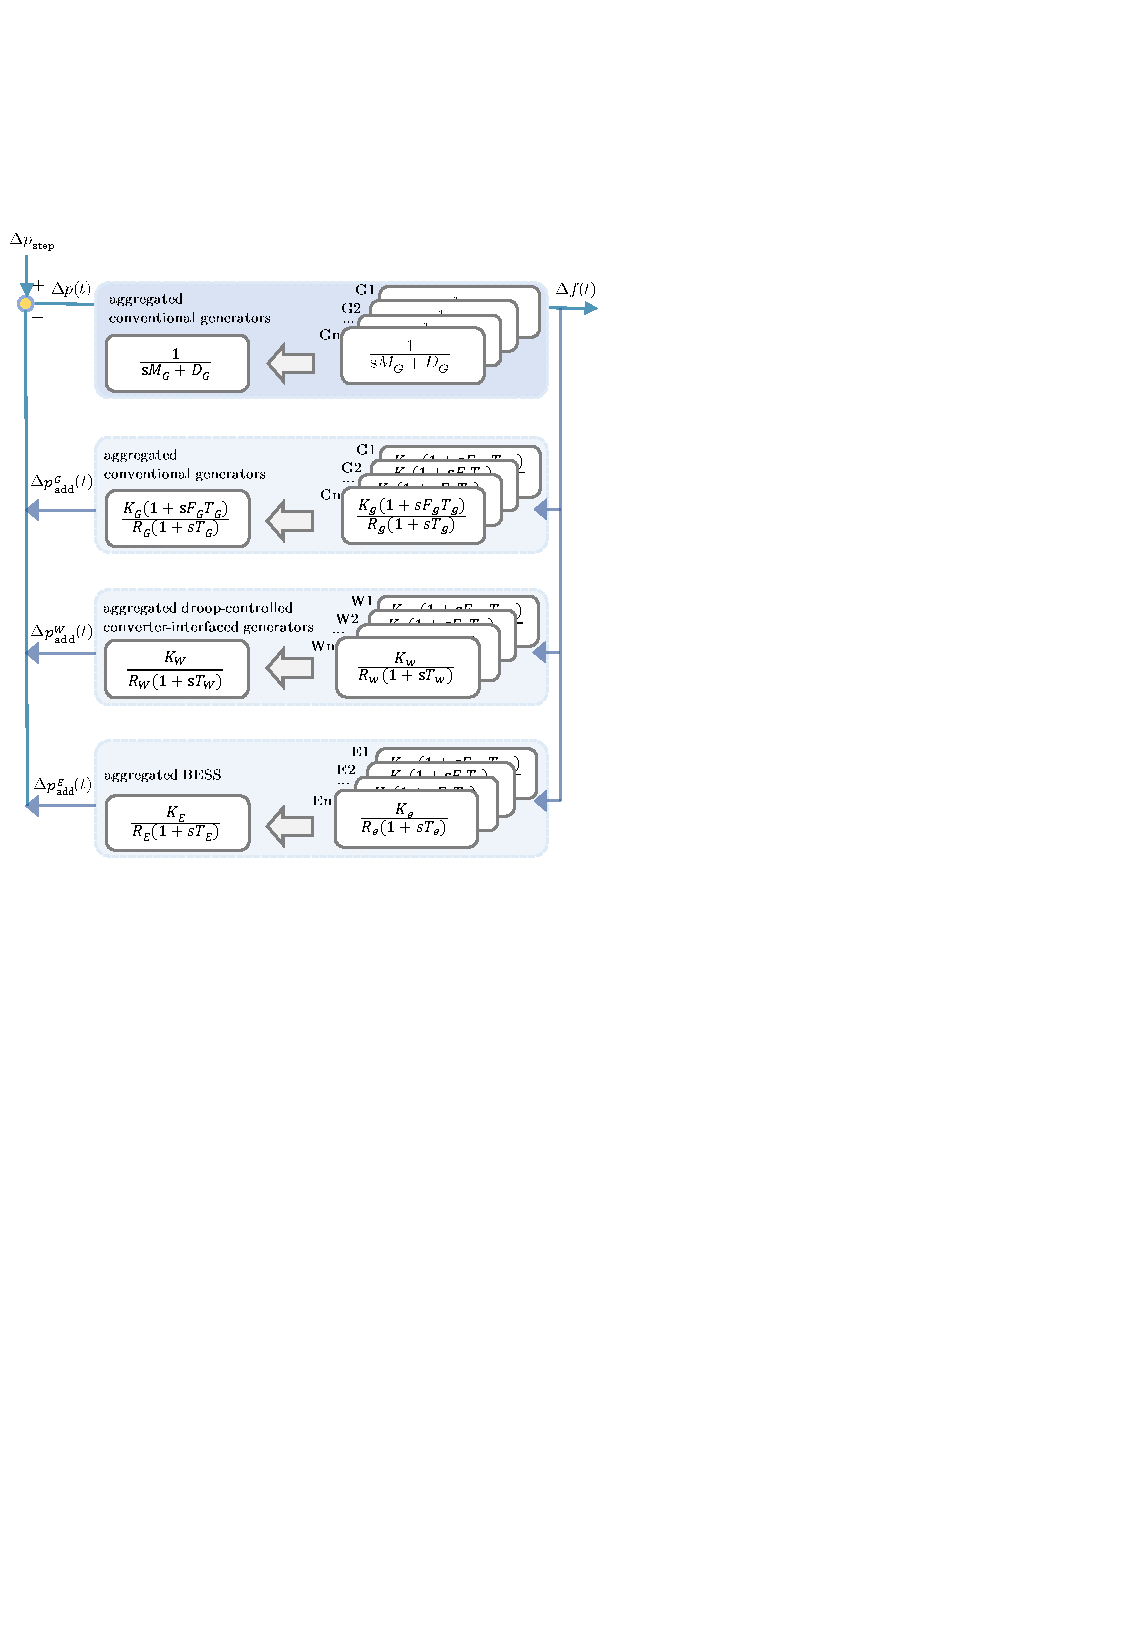
\includegraphics[width=0.9\linewidth, height = 3.in]{fig1}
%    \caption{The unified frequency dynamic response of electrical power systems against occurred power disturbance}
%    \label{fig1}
%\end{figure}

\noindent where \cref{eqn:2a,eqn:2b} describes the chronological change of \(\varDelta f(t)\) over the entire dynamic horizons; \cref{eqn:2c} denotes equivalent frequency parameters consisting of CoI-based inertia constant and droop constant; \cref{eqn:2d,eqn:2e,eqn:2c} describes the scheduled output of different generators,  respectively. Furthermore, by replacing $\varDelta f^{\prime}(t) = \nicefrac{[\varDelta f(t)-\varDelta f(t-\delta t)]}{ \delta t}$ into \cref{eqn:2a,eqn:2d}, the time-discretized SFR concerning $\varDelta f(t)$, as well as rescheduled output \(\langle \varDelta p_{G}(t), \varDelta p_{W}(t)\rangle\) from conventional generators and converter-interfaced ones can be estimated,

% \vspace{-0.125in}
\begin{newsubequations}\label{eqn:3}
	\begin{align}
		 & \varDelta f(t) = \frac{1}{2}{H_{\varSigma}^{-1}}\varDelta p(t) \delta t - \left(1 - \frac{1}{2}{D_{\varSigma}}{H_{\varSigma}^{-1}}\right)\varDelta f(t-\delta t) \delta t   \label{eqn:3a} \\
		 & \varDelta p_{G}(t)={K_{G} }{ R_{G}^{-1}} \varDelta f(t) - \varLambda \int_{0}^{t} e^{\frac{1}{T_G}(t)} \cdot \label{eqn:3b}                                                                \\
		 & \qquad \left(\varDelta f(t) - \varDelta f(t-\varDelta t) \right) d t: \varLambda = {K_G(1-F_G)}{ R_{G}^{-1} }e^{-\frac{1}{T_G} (t)} \notag                                                 \\
		 & \varDelta p_{W}(t) = \left({K_{W} } R_{W}^{-1} \!+\! D_{W} \!+\! 2H_{W} \delta t\right) \varDelta f(t) -\notag                                                                             \\
		 & \qquad \quad \qquad 2H_{W} \delta t \varDelta f(t - \delta t)  \label{eqn:3c}
	\end{align}
\end{newsubequations}

% By implementing the inverse Laplace transformation in (1) and reshaping it as related differentiable form, the time-discretized expression of frequency dynamic can be derived as (1). More details on the derivatives of frequency response from s-domain to t-domain can be found int the appendix I.

% \vspace{-0.125in}
% \begin{newsubequations}\label{eqn:3}
%   \begin{align}
%     \varDelta f(t + \delta t) & =\varDelta f(t)+(2H_{{e}})^{-1}\bigl(\varDelta p(t)-D_{{e}} \varDelta f(t)\bigr)  \label{time-discretized SFR: swing equation}                                                                                                     \\
%     \varDelta p(t)            & =\varDelta p_{{step}}-\varDelta p_{G}(t)-\varDelta p_{W}(t)-\varDelta p_{E}(t) \label{time-discretized SFR: mismatch power}                                                                                                        \\
%     \varDelta p_{G}(t)        & ={K_{G} }{ R_{G}^{-1}} \varDelta f(t)- \left({K_G(1-F_G)}{ R_{G}^{-1} }e^{-\frac{1}{T_G} (t)}\right) \int_{0}^{t}  e^{\frac{1}{T_G}t} \varDelta f(t)\delta t\label{time-discretized SFR: additional power from convertional units} \\
%     \varDelta p_{W}(t)        & ={ R_{W}^{-1} } \varDelta f(t) \label{time-discretized SFR: additional power from converters}                                                                                                                                      \\
%     \varDelta p_{E}(t)        & ={ R_{E}^{-1} } \varDelta f(t) \label{additional power from bess}
%   \end{align}
% \end{newsubequations}

In \cref{eqn:3b,eqn:3c}, \(\langle \varDelta p_{G}(t), \varDelta p_{W}(t) \rangle\) can be recursively calculated after observing \(\varDelta f(t\!-\! \delta t)\) and \(\varDelta f(t)\). Nevertheless, the impact of uncertain variability factors is implicitly ignored. Generally speaking, uncertain variability factors are divided into two parts; the first part comes from the restriction of \(\varDelta p_{G}(t)\) denoted by \(\overline{p}_{G},\overline{p}_{W}\), it means that the adjustable output of generators using \cref{eqn:3b,eqn:3c} cannot be kept due to generators' output limitation; the latter part is caused by the unforeseeable uncertain derivations produced by intermittent converter-interfaced generators. To address that, let \(\varDelta \omega_{1}(t)\!=\!-\left(\lceil \varDelta p_{G}(t), \overline{p}_{G} \rceil \!+\! \lceil \varDelta p_{W}(t), {p}_{W}(t)\rceil\right)  \) represent the corrected term caused by generators' output limitation, and similarly, let \(\varDelta \omega_{2}(t)=\textrm{Normal}(t; \mu, \sigma)\) denote uncertain derivations from converter-interfaced generators. Hence, the impact of uncertain variability factors can be estimated by adding \(\varDelta \omega_{1}\) and \(\varDelta \omega_{2}\) together. So, the SFR considering uncertain variability factors can be derived,

% \vspace{-0.125in}
\begin{newsubequations}\label{eqn:4}
	\begin{align}
		\varDelta f(t) = & \frac{1}{2}{H_{\varSigma}^{-1}}\varDelta p(t) \delta t - \left(1 - \frac{1}{2}{D_{\varSigma}}{H_{\varSigma}^{-1}}\right)\varDelta f(t-\delta t) \delta t + \notag \\
		                 & \varDelta\omega: \varDelta \omega =\varDelta \omega_{1}(t) + \varDelta \omega_{2}(t)
		% \varDelta \omega_{1}(t)\!=\!-\left(\lceil \varDelta p_{G}(t), \overline{p}_{G} \rceil \!+\! \lceil \varDelta p_{W}(t), \overline{p}_{W}\rceil\right), \varDelta \omega_{2}(t)=\textrm{Normal}(t; \mu, \sigma), \label{eqn:4a}
	\end{align}
\end{newsubequations}

The stochastic differential equation (SDE) defined in \cref{eqn:4} does not have an analytical solution due to the independence between uncertain variability factors and \(\varDelta f(t)\). To solve this, a Bayesian filter framework is introduced to estimate the posterior distribution of \(\varDelta f(t)\). Let \(\mathcal{P} (\varDelta f(t)), \mathcal{P}(\varDelta p(t))\), respectively, enforces the probabilistic density distribution of \(\varDelta f(t)\) and \(\varDelta p(t)\), then, the posterior distribution of \(\varDelta f(t)\) can be estimated by,

% \(\varDelta f(t) \Rightarrow \varDelta f(t + \delta t)\) enforce a hidden Markov decision process, and \(\varDelta p(t) \Rightarrow \varDelta p(t+\delta t)\) be a measured state observable process, \(\varDelta f(t + \delta t)\) can be solved alternately, as illustrated in figure.(2).

% \begin{table*}[b]\vspace{-0.25cm}
% 	\normalsize
% 	\rule{1.0\textwidth}{.05pt}
% 	\vspace{-0.5cm}
% 	\begin{align}\label{eqn:4}
% 		 & \mathcal{P}\left(\varDelta f(t_0+ (n+ 1)\delta t) \mid \varDelta p\left(t_{0}: t_0+ (n+ 1)\delta t\right), u_{1}, \sigma_{1}\right) =                                                                                                                                                                                                                                  \\
% 		 & \qquad \frac{\mathcal{P}\left(\varDelta f(t_0+ (n+ 1)\delta t) \mid \varDelta p\left(t_{0}: t\right), u_{1}, \sigma_{1}\right) \mathcal{P}\left(\varDelta p(t_0+ (n+1)\delta t) \mid \varDelta f(t_0+(n+ 1)\delta t), u_{1}, \sigma_{1}\right)}{\mathcal{P}\left(\varDelta p(t_0+(n+1)\delta t) \mid \varDelta p\left(t_{0}: t\right), u_{2}, \sigma_{2}\right)}\notag
% 	\end{align}
% 	% \hspace{0.5\textwidth}\rule{0.5\textwidth}{.4pt}
% \end{table*}

\begin{newsubequations}\label{eqn:5a}
	\begin{align}
		 & posterior: \mathcal{P}(\varDelta f(t)\! | \varDelta p(t_0\!:\! t); \varDelta \omega)\!=\!\underbrace{\mathcal{P}(\varDelta p(t) | \varDelta f(t); \varDelta\omega)}_{\textrm{\textit{likelihood function}}}\\
		 &\qquad \underbrace{\mathcal{P}(\varDelta f(t) | \varDelta p(t_0\!:\! t\!-\!\delta t); \varDelta \omega)}_{\textrm{\textit{prior function}}} { {\mathcal{P}^{-1}(\varDelta p(t) | \varDelta p(t_0\!:\! t\!-\!\delta t);\varDelta \omega)}}\notag
	\end{align}
\end{newsubequations}
% \annotate[yshift=1em]{above}{k1}{normalization factor}
% \annotate[yshift=1em]{below}{k2}{prior probabilistic distribution}
% \annotate[yshift=1em]{below}{k3}{likelihood function}

% \noindent where \cref{time-discretized SFR: swing equation} declares the change of $\varDelta f(t)$ between adjacent discretized steps; \cref{time-discretized SFR: mismatch power} describes the evolution of mismatch power. \cref{time-discretized SFR: additional power from conventional units,time-discretized SFR: additional power from converters,additional power from bess}  represent additional regulated outputs produced by aggregated conventional generators, aggregated wind farms and aggregated BESS.

\noindent where \(\textit{likelihood function}\) in \eqref{eqn:5a} declares coupling properties between \(\varDelta p(t)\) and \(\varDelta f(t)\); and \(\textit{prior function}\) describes the sequential recursive process from \(\varDelta f(t_0: t-\delta t)\) to \(\varDelta f(t)\). Using the prior and predicated processes of the Bayesian filter written probabilistically, the impact of uncertain variability factors denoted by \(\varDelta \omega\) can be well incorporated over the entire frequency dynamic process.
In which, \(\textit{prior function}\) can be recursively calculated as follows,

% \vspace{-0.125in}
\begin{newsubequations}\label{eqn:6a}
	\begin{align}
		 & prior: \mathcal{P}\left(\varDelta f(t) \!\mid\!  \varDelta p\left(t_{0}: t-\delta t \right), \varDelta \omega\right) =\int \bigl(\mathcal{P}(\varDelta f(t) \!\mid\! \\
		 & \varDelta f(t_0:t-\delta t), \varDelta \omega) \cdot
		\mathcal{P}\!\left(\varDelta \!f(t-\delta t) \!\mid\!  \varDelta p\!\left(t_{0}\!: \! t-\delta t\right), \varDelta \omega\right) \bigr) d \varDelta f(t) \notag
	\end{align}
\end{newsubequations}

% \(\mathcal{P}(\varDelta f(t) \mid \varDelta p\left(t\right), \varDelta \omega)\)  can be estimated by estimating its prior form $\mathcal{P}\left(\varDelta f(t) \!\mid\! \varDelta p\left(t_{0}\!: \! t-\delta t \right), \varDelta \omega \right)$ and a normalized constant $\mathcal{P}\left(\varDelta p(t) \mid \varDelta f\left(t\right), \varDelta \omega \right)$, with their forms can be found in \cref{eqn:5}.

% Previous studies generally adhere to a free residual assumption and have provided evidence that $\varDelta f(t)$ can be achieved by either an analytical closed-form solution \cite{anderson1990low, shi2018analytical, markovic2018lqr, ye2015analytical, mercier2009optimizing, paturet2020stochastic} or a time-discretized solution \cite{vatani2015relay, oskouee2021primary, pena2018voltage, zhao2020frequency}. In contrast to previous studies that have been discussed, the BF-SFR approach incorporates the influence of residual representing UV issue. The significance of UV is understood in two main aspects: $i$) the intermittent characteristic of converter-interfaced generators participating in frequency support, leading to the inevitable residual relative to the ideal value; $ii$) potential measured residuals are due to aging behavior or aberrant operation of electrical devices. By formulating the SFR considering residual factors as a hidden Markov decision process (see Fig.~\ref{fig2}), it becomes possible to estimate the posterior distribution of $\varDelta f(t)$ using a recursive mathematical formulation.

% Since $\varDelta p_{a d d}^{G}, \varDelta p_{a d d}^{W}$ and $\varDelta p_{a d d}^{E}$ are independent on aggregated frequency dynamic parameters and previous frequency derivation.

% Let $\mathcal{P}\left(\varDelta f(t_0 \!+\!n\delta t), \mu_{1}, \sigma_{1}\right)$ represents the posterior PDF of $\varDelta f(t_0\! +\! n \delta t)$ at the $n\!-\!th$ discretized step; $\mathcal{P}(\varDelta p(t_0 \!+\!n \delta t), $ $\mu_{2}, \sigma_{2})$ denotes the posterior PDF of $\varDelta p(t_0 \!+\! n \delta t)$ at the $n\!-\!th$ discretized step. $\langle\mu_{1}, \sigma_{1}\rangle$, $\langle\mu_{2}, \sigma_{2}\rangle$, respectively, denote the expectation and variance of residuals in the observation process and measured process. $\mathcal{P}\left(\varDelta f(t_0\!+\!(n\!+\!1)\delta t)\mid \varDelta p(t_{0}: t_0+\right.$ $\left. (n\!+\! 1)\delta t\right), $ $u_{1}, \sigma_{1})$ to denote a conditional distribution of $\mathcal{P}(\varDelta f(t_0+(n+1)\delta t), $ $u_{1}, \sigma_{1})$, It describes that the posterior of $\mathcal{P}(\varDelta f(t_0 +(n+1)$ $\delta t), u_{1}, \sigma_{1})$ can be fully inferred after obtaining all measured sequences $\varDelta p\left(t_{0}: t_0+(n+1)\delta t\right)=\{\varDelta p_{t} \mid t \in[t_{0}, t_0+(n+1)\delta t]\}$. Its mathematical formulation can be derived as \cref{eqn:4} according to the Bayesian theorem.

\begin{figure}[!t]\vspace{-0.1in}
	\centering
	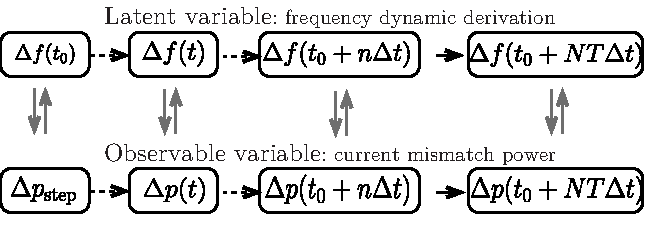
\includegraphics[width=0.8\linewidth, height=0.95in]{fig2}
	\caption{The discretized recurrence process of frequency derivation in the proposed BF-SFR method}
	\label{fig2}
\end{figure}

% Next, let the initial time $t_{0} = 0$ and replace $\langle \varDelta f(t_0 \!+\! n \delta t)\rangle$, $\langle \varDelta p(t_0 \!+\! n\delta t) \rangle$ with their abbreviated forms $\left\langle \varDelta f(n),\varDelta p(n)\right\rangle$, \cref{eqn:5} can be further simplified as follows,

% \vspace{-0.125in}
% \begin{newsubequations}\label{eqn:6}
% 	\begin{align}
% 		 & \mathcal{P}\left(\varDelta f(n+1) \!\mid\! \varDelta p\left(0: n\right), u_{1}, \sigma_{1}\right)= \int \bigl\{\mathcal{P}(\varDelta f(n+1) \mid \bigr. \label{eqn:6a}                              \\
% 		 & \qquad\quad \bigl. \varDelta f(n), \left.u_{1}, \sigma_{1}\right) \mathcal{P}\left(\varDelta f(n) \!\mid\!  \varDelta p\left(0: n\right), u_{1}, \sigma_{1}\right)\bigr\} d \varDelta f(n+1) \notag \\
% 		 & \mathcal{P}\left(\varDelta p(n+1) \!\mid\!  \varDelta p\left(0: n\right), u_{2}, \sigma_{2}\right)=  \int \bigl\{\mathcal{P}(\varDelta p(n+1)\!\mid\! \bigr. \label{eqn:6b}                         \\
% 		 & \bigl. \varDelta f(n+1)\left.u_{2}, \sigma_{2}\right) \mathcal{P}\left(\varDelta f(n+1) \!\mid\!  \varDelta p\left(0: n\right), u_{2}, \sigma_{2}\right) \bigr\}d \varDelta f(n+1)\notag
% 	\end{align}
% \end{newsubequations}

In \cref{eqn:5a,eqn:6a}, \textit{prior function} and \textit{posterior function} can not be directly solved because their distributional types and expressions are unknown. Therefore, a sequential importance sampling (SIS) algorithm is applied here to address this issue. 
Let \(\mathcal{Q} (\varDelta f(t) | \varDelta p(t_0\!:\!t);\varDelta \omega)\) denote the importance density, which can be treated as the replaceable proposed function for generating samples (filters); and \(\lambda (\varDelta f(t_0:t))\) describes the importance weight, which are approximations to the posterior probabilistic of the samples following \eqref{eqn:7a}, then, \eqref{eqn:6a} can be estimated as the product between the importance density and weight, 

\vspace{-0.125in}
\begin{newsubequations}\label{eqn:7}
	\begin{align}
		&\!\!\!\!\!\!\!\!\!\!\!\!\!\!\!\!\!\!\!\!\!\!\! \mathcal{P}(\varDelta f(t)|\varDelta p(t_0\!:\!t);\varDelta \omega)=\label{eqn:7a}\\
		&\quad \mathcal{Q}(\varDelta f(t)|\varDelta p(t_0\!:\!t);\varDelta \omega) \cdot \lambda (\varDelta f(t_0:t))\notag\\
		{weight}: &\lambda (\varDelta f(t_0:t)) = \frac{\mathcal{P} (\varDelta f(t) | \varDelta p(t_0\!:\!t);\varDelta \omega)}{\mathcal{Q} (\varDelta f(t) | \varDelta p(t_0\!:\!t);\varDelta \omega)} \label{eqn:7b}\\
		density: &\mathcal{Q} (\varDelta f(t) | \varDelta p(t_0\!:\!t);\varDelta \omega) = \mathcal{Q}(\varDelta f(t)|\varDelta f(t_0\!:\!t\!-\!\delta t); \varDelta \omega)\cdot \notag\\
		&\mathcal{Q}(\varDelta f(t-\delta t)|\varDelta p(t_0\!:\!t-\delta t);\varDelta \omega)  \label{eqn:7c}
	\end{align}
\end{newsubequations}

By supposing the recursive type of the importance density and sequentially transferring it as \eqref{eqn:7c}, the similar recursive form of importance weight can be derived as,

\vspace{-0.125in}
\begin{newsubequations}
	\begin{align}
		&\textit{recursive weight}: \lambda(\varDelta f(t_0\!:\!t)) = \lambda(\varDelta f(t_0\!:\!t\!-\!\delta t))\cdot \label{eqn:8a}\\ 
		&\qquad \mathcal{P}(\varDelta p(t)|\varDelta f(t_0\!:\!t);\varDelta \omega)\left(\frac{\mathcal{P}(\varDelta f(t)|\varDelta f(t_0\!:\!t-\delta t);\varDelta \omega)}{\mathcal{Q}(\varDelta f(t)|\varDelta f(t_0\!:\!t-\delta t);\varDelta \omega)}\right) \notag
	\end{align}
\end{newsubequations}

Let \(\mathcal{Q}(\varDelta f(t)|\varDelta f(t_0\!:\!t-\delta t);\varDelta \omega)\) equals to the transfer function \(\mathcal{P}(\varDelta f(t)|\varDelta f(t_0\!:\!t-\delta t);\varDelta \omega)\), and then, \eqref{eqn:8a} can be rewritten as,

\begin{newsubequations}
	\begin{align}
		&\lambda(\varDelta f(t_0\!:\!t)) = \lambda(\varDelta f(t_0\!:\!t\!-\!\delta t))\cdot 
		\mathcal{P}(\varDelta p(t)|\varDelta f(t_0\!:\!t);\varDelta \omega)\label{eqn:9a}
	\end{align}
\end{newsubequations}

By combining \eqref{eqn:9a} and \eqref{eqn:7a}, the posterior of the importance density concerning \eqref{eqn:7c} can be directly derived. Subsequently, by updating the weight through \eqref{eqn:7b} and sequentially substituting \cref{eqn:7b,eqn:7c} into \eqref{eqn:7a}, the posterior distribution of \(\varDelta f(t)\) concerning \eqref{eqn:5a} can be recursively solved. For intuitively illustrating the implementing process of the posterior distribution of \(\varDelta f(t)\). 


% To calculate the posterior function of $\mathcal{P}(\varDelta f(n\!+\!1) \! \mid\! \varDelta p(0 \!:\! n),$ $ u_{1}, \sigma_{1})$ and $\mathcal{P}(\varDelta p(n\!+\!1) \!\mid\! \varDelta p(0\!:\!n), u_{2}, \sigma_{2})$, the operator $\!\!\int(\cdot)\!\!$  in \eqref{eqn:5} can be approximately estimated by an expectation of a certain number of sampled data (or called $filters$), i.e., $\int\varpi[\varDelta f(n)] d\varDelta f(n) \!\approx\! \frac{1}{N}$ $ \sum_{n=1}^{N} \varpi\left(\lambda_{n}\right) \lambda_{n}$ where $\varpi$ enforces associated integrated function in \eqref{eqn:6} and $\lambda_{n}$ represents possible $filters$ generated from the prior of $\varDelta f(n)$. Hence, \eqref{eqn:6} can be rewritten as,


% \vspace{-0.125in}
% \begin{newsubequations}\label{eqn:7}
% 	\begin{align}
% 		 & \mathcal{P}\left(\varDelta f(n\!+\!1) \!\mid\! \varDelta p\left({0}\!:\! n\right), u_{1}, \sigma_{1}\right)\!= \label{eqn-7: sequential relation of adjacent frequency derivations} \\
% 		 & \quad N^{-1}\sum\nolimits_{n=1}^{N} \mathcal{P}\left(\varDelta f(n+1) \mid \varDelta f(n), u_{1}, \sigma_{1}\right)\lambda_{n}^{\prime}\notag                                       \\
% 		 & \mathcal{P}\left(\varDelta p(n\!+\!1) \!\mid\! \varDelta p\left({0}\!:\! n\right), u_{2}, \sigma_{2}\right) \!=\label{eqn-7: sequential relation of adjustable outputs}             \\
% 		 & \quad N^{-1}\sum\nolimits_{n=1}^{N} \mathcal{P}\left(\varDelta p(n+1) \mid \varDelta f(n+1), u_{2}, \sigma_{2}\right)\lambda_{n}^{\prime\prime} \notag                              \\
% 		 & \lambda_{n}^{\prime} = \mathcal{P}\left(\varDelta f(n) \!\mid\!  \varDelta p\left(0: n\right), u_{1}, \sigma_{1}\right)\notag                                                       \\
% 		 & \lambda_{n}^{\prime\prime} = \mathcal{P}\left(\varDelta f(n+1) \!\mid\!  \varDelta p\left(0: n\right), u_{2}, \sigma_{2}\right)\notag
% 	\end{align}
% \end{newsubequations}

% \noindent where $\lambda^{\prime}, \lambda_{n}^{\prime \prime}$, respectively, represent random filters following associated integrated functions in (7b) and (7d). In combination with \eqref{eqn-7: sequential relation of adjacent frequency derivations} and \eqref{eqn-7: sequential relation of adjustable outputs}, the posterior probabilistic assessment of $\varDelta f(n+1)$ concerning $\mathcal{P}(\varDelta f(n+1))$ can be carried out with the below steps:
% \begin{itemize}
% 	\item[$\,\,i)$ ] \textit{Bayesian inference} in the prior stage, here, \eqref{eqn-7: sequential relation of adjacent frequency derivations} is used to generate \textit{filters} to capture the likely value of $\varDelta f(n+1)$;
% 	\item[$ii)$] \textit{Bayesian predication} in the prediction stage, \eqref{eqn:4} and \eqref{eqn-7: sequential relation of adjuctable outputs} is used to update the posterior of $\varDelta f(n+1)$. Since $\lambda^{\prime}, \lambda_{n}^{\prime \prime}$ cannot directly be generated from $\mathcal{P}\left(\varDelta f(n) \!\mid\! \varDelta p\left(0\!:\! n\right), u_{1},\right.$ $\left. \sigma_{1}\right)$ and $\mathcal{P}\left(\varDelta f(n\!+\!1) \!\mid\! \varDelta p\left(0\!:\!\right.\right.\left.n), u_{2}, \sigma_{2}\right)$ because their functions are unknown, Therefore, sequential Important Sampling (SIS) method is used to calculate the integrated functions. Especially, $\mathcal{P}(\varDelta f(n) \!\!\mid\!\! \varDelta p(0\!:\! n), \!u_{1},\!\sigma_{1})$ at the $n\!-\!th$ prior stage is taken as an example to describe the calculating process using SIS, the case of the latter (posterior) stage concerning $\mathcal{P}\left(\varDelta f(n+1) \!\mid\! \varDelta p\left(0: n\right), u_{2}, \sigma_{2}\right)$ is in a similar solution.
% \end{itemize}

% Let $\iota(n)\!=\!\mathcal{P}\left(\varDelta f(n) \!\mid\! \varDelta p\left({0}: n\right), u_{2}, \sigma_{2}\right), \iota(n)=(\nicefrac{\iota(n)}{ \lambda(n)}) \!\cdot\! \lambda(n)$ where $\iota(n)$ is the original probabilistic density function of posterior distribution at $t\!\! = \!\!n \delta t$; $\lambda(n)$ enforces a proposed function. $\gamma(n) \!=\! \nicefrac{\iota(n)}{\lambda(n)}$ represents a likelihood coefficient. Hence, the \!$filters$\! following $\iota(n)$ can be alternatively sampled from $\lambda(n)$ with a related weight coefficient $\gamma(n)$, i.e., $\iota(n) = $ $\lambda (n)\gamma(n)$.

% \vspace{-0.125in}
% % \begin{table}[b]\normalsize
% % \rule{1.0\textwidth}{.1pt}
% \begin{small}
% 	\begin{align}\label{eqn:8}
% 		 & \gamma(n\!+\! 1)=
% 		\frac{\iota(\varDelta f(n\!+\!1)|\varDelta p(0\!:\!n\!+\!1),\mu_1,\sigma_1)}{\lambda(\varDelta f(n\!+\!1)|\varDelta p(0\!:\!n\!+\!1),\mu_2,\sigma_2)}=\gamma(n)\times                                                                     \\
% 		 & \qquad\,\, \left(\frac{\iota(\varDelta f(n\!+\!1)|\varDelta f(t),\!\mu_1,\!\sigma_1)\iota(\varDelta p(n\!+\!1)|\varDelta f(n\!+\!1),\!\mu_2,\!\sigma_2)}{\lambda(\varDelta f(n\!+\!1)|\varDelta f(t),\!\mu_1,\!\sigma_1)}\right)\notag
% 	\end{align}
% \end{small}
% % \hspace{0.5\textwidth}\rule{0.5\textwidth}{.4pt}
% % \end{table}
% % \begin{table*}[b]\normalsize
% % \rule{1.0\textwidth}{.1pt}
% % \begin{align}\label{eqn:8}
% % &\gamma(n+1)=
% % \frac{\iota(\varDelta f(n+1)|\varDelta p(0:n+1),\mu_1,\sigma_1)}{\lambda(\varDelta f(n+1)|\varDelta p(0:n+1),\mu_2,\sigma_2)}=\\
% % &\qquad \frac{\iota(\varDelta f(n+1)|\varDelta f(n),\mu_1,\sigma_1)\iota(\varDelta p(n+1)|\varDelta f(\varDelta p(n+1),\mu_2,\sigma_2)\iota(\varDelta p(n+1)|\varDelta f(\varDelta p(n+1),\mu_2,\sigma_2)}{\lambda(\varDelta f(n+1)|\varDelta f(n),\mu_1,\sigma_1)\lambda(\varDelta f(n)|\varDelta p(0:n),\mu_1,\sigma_1)}=\notag\\
% % &\qquad \gamma(n)\left(\frac{\iota(\varDelta f(n+1)|\varDelta f(t),\mu_1,\sigma_1)\iota(\varDelta p(n+1)|\varDelta f(n+1),\mu_2,\sigma_2)}{\lambda(\varDelta f(n+1)|\varDelta f(t),\mu_1,\sigma_1)}\right)\notag
% % \end{align}
% % % \hspace{0.5\textwidth}\rule{0.5\textwidth}{.4pt}
% % \end{table*}

% Substituting $\iota(n+1) = \lambda (n+1)\gamma(n+1), \iota(n) = \lambda (n)\gamma(n)$ into \eqref{eqn:4}, $\iota(n+1)$ can be recursively calculated through \eqref{eqn:8}. In \eqref{eqn:8}, another critical issue to be reviewed is the selection of the proposed distribution. Here, the recursive transfer distribution $\iota(\varDelta f(n+1)|\varDelta f(n),\mu_1,\sigma_1)$ can be used to simplify the calculation process. Accordingly, the updating weight \eqref{eqn:8} can be reduced as,

% \vspace{-0.125in}
% \begin{align}\label{eqn:9}
% 	 & \gamma(n+1)=
% 	\gamma(n)\iota(\varDelta p(n+1)|\varDelta f(n+1),\mu_2,\sigma_2)
% \end{align}

% In \eqref{eqn:9}, the likelihood rate in each iteration can be recursively derived from $\iota(\varDelta p(n+1)|\varDelta f(n+1),\mu_2,\sigma_2)$. On this basis, let $\langle \varDelta f^{(n)}(t+(n+1)\delta t), \left( \varDelta p\right)^{(n)}(t+(n+1)\delta t)\rangle$ define the sampled \textit{filters} from the pro-selected proposed function $\lambda^{\prime}(n+1)$ in the inference stage and $\lambda^{\prime\prime}(n+1)$ in the predication stage; $\langle\gamma^{\prime}(n+1),\gamma^{\prime\prime}(n+1)\rangle$ represent the likelihood rate at $t\!=\! t_0 + (n+1)\delta t$ at these two stages. Table \ref{table: modeling BF-SFR} describes the Pseudo-Code of the proposed BF-SFR method.


% \begin{table}[!t]\vspace{-0.250in}
% 	\caption{The simulation of BF-SFR through SIS algorithm}\label{table: modeling BF-SFR}
% 	\begin{tabular}{cl}
% 		\hline
% 		NO. & \qquad\qquad\qquad\qquad Calculation processes                                                                                     \\
% 		\hline
% 		1   & \textbf{Initialize}: $\text{Discretized step}\,\, \delta t \!= \!0.05 s$; Initialized time $t_0 \!=\! 0s$                          \\
% 		    & \qquad \qquad\,  $\text{Counter}$\, $n$ = 0; \text{Filter number} \, $NT$ = 1000                                                   \\
% 		2   & \textbf{For}\,\, $n = 0$, \textbf{Then}                                                                                            \\
% 		3   & \quad\textbf{Let} $t=t_0+\delta t\times n$, \textbf{Then}                                                                          \\
% 		4   & \qquad \textbf{Inference process}:                                                                                                 \\
% 		    & \qquad Generating possible (instant) filters                                                                                       \\
% 		    & \qquad $\left(\varDelta f\right)^{(n)}(t_0 \!+ \!(n\!+\!1) \delta t)$  from proposed distribution:                                 \\
% 		    & \qquad $\lambda^{\prime}(n+1)\sim\mathcal{P}(\varDelta f(t_0\!+\!(n\!+\!1)\delta t)| \varDelta p(t_0\!:\!t_0 \!+\! n\delta t),$    \\
% 		    & \qquad $\mu_1,\sigma_1)$ in \eqref{eqn:6a};                                                                                        \\
% 		5   & \qquad  \textbf{Prediction process}:                                                                                               \\
% 		    & \qquad Generating possible observation filters                                                                                     \\
% 		    & \qquad $\left(\varDelta p\right)^{(n)}(t_0 \!+\! (n\!+\!1)\delta t)$ from normalized distribution:                                 \\
% 		    & \qquad  $\lambda^{\prime\prime}(n+1)\sim\mathcal{P}(\varDelta p(t_0\!+\!(n\!+\!1)\delta t)| \varDelta p(t_0:t_0 \!+\! n\delta t),$ \\
% 		    & \qquad $\mu_2,\sigma_2)$ in \eqref{eqn:6b};                                                                                        \\
% 		6   & \qquad \textbf{Updating weight coefficients:}                                                                                      \\
% 		    & \qquad Calculating $\gamma^{\prime}\,\text{and}\, \gamma^{\prime\prime}$ through \eqref{eqn:9}, and                                \\
% 		    & \qquad Re-estimate original filters $\left(\varDelta f\right)^{(n)}(t_0 \!+ \!(n\!+\!1) \delta t)$ via \eqref{eqn:4}               \\
% 		7   & \quad \textbf{End Let}                                                                                                             \\
% 		8   & \textbf{End For}                                                                                                                   \\
% 		\hline
% 	\end{tabular}
% \end{table}

\vspace{-0.100in}
\section{Frequency constraint reformulation}
\vspace{-0.0250in}

This section examines the represented criteria of frequency dynamic requirements, including RoCoF, nadir, and frequency containment reserve (FCR). These needs are reevaluated and integrated into the restrictions considered in UC problems. Fig. \ref{fig3} visualizes the physical significance of these feature criteria. Remarkably, the reconstructed chance-constrained frequency nadir constraint is derived from the proposed BF-SFR approach derived in section II, other constraints related to RoCoF and FCR can be found in \cite{restrepo2005unit, teng2015stochastic, chu2020towards, ding2021two,zhang2020modeling, zhang2021encoding,oskouee2021primary,perroy2019provision,wang2021adaptive}.

\vspace{-0.225in}
\subsection{$RoCoF \,\,constraint$}
\vspace{-0.0125in}
%To prevent $\varDelta f(t)$ from changing too fast at inertia response, the differential of frequency derivation $\varDelta f(t)$, denoted by $\varDelta f^{\prime}(t)$, is included, i.e., $\varDelta f^{\prime}(t)\leq RoCoF_{\text{max}}$. Since $\varDelta f^{\prime}(t)$  $=\nicefrac{\varDelta p_{\text{step} }}{M_{\text{equ}}}: M_{\text{equ}} = M_G+M_{W}$, the $RoCoF$ constraint can be obtained,

To mitigate rapid changes in the inertia response, the change of RoCoF, indicated as $\varDelta f^{\prime}(t)$, is necessary. It is required that $\varDelta f^{\prime}(t)$ does not exceed the maximum rate of change of frequency, denoted as $RoCoF_{\text{max}}$, \textit{i.e.,} $\varDelta f^{\prime}(t)\!\leq \! RoCoF_{\text{max}}$. Since $\max\{\varDelta f^{\prime}(t)\}=\nicefrac{\varDelta p_{\text{step} }}{M_{\text{equ}}}:\! M_{\text{equ}} \!=\! M_G\!+\!M_{W}$, \cite{garcia2021requirements}, associated $RoCoF$ constraint can be obtained,

\vspace{-0.125in}
\begin{small}
	\begin{align}\label{eqn:10}
		 & \slfrac{\varDelta p_{\text{step} }}{M_{\text{equ} }}\leq RoCoF_{\text{max}}                                                                                                                   \\
		 & \quad\,\,\,\Longleftrightarrow M_{G} \!\geq\! \slfrac{\varDelta p_{\text{step} }}{RoCoF_{\text{max} }} \!-\! M_W, \forall g, t  \notag                                                        \\
		 & \quad\,\,\,\Longleftrightarrow \sum\nolimits_{g=1}^{NG}M_{g}x_{g,t} \!\geq\! \frac{\varDelta p_{\text{step} }}{RoCoF_{\text{max} }} \!-\! \sum\nolimits_{w=1}^{NW} M_{w}, \forall g, t \notag
	\end{align}
\end{small}

\vspace{-0.15in}
\subsection{$FCR \,\,constraint$}

\begin{figure}[!t]\vspace{-0.25cm}
	\centering
	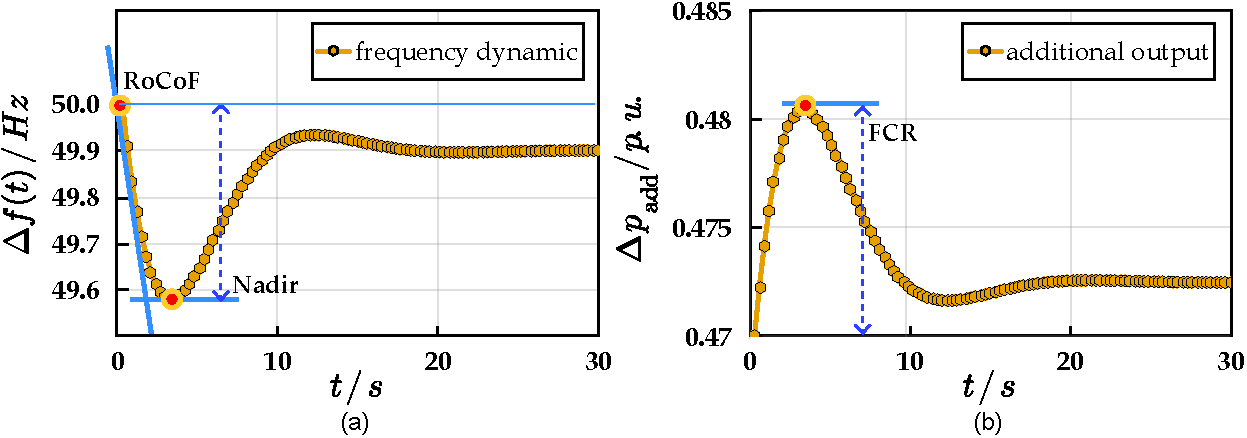
\includegraphics[width=1.0\linewidth]{fig3}
	\caption{Three frequency dynamic requirements: $RoCoF$, $nadir$ and $FCR$}
	\label{fig3}
\end{figure}

To guarantee sufficient frequency reserve provided by grid-connected units, conventional generators, converters, and BESS must be capable of serving as reserves during imbalanced disturbances, \cite{zhang2020modeling,9964327}. In combination with (3), the binding of the additional power $\langle \varDelta p_{add}^{G}, \varDelta p_{add}^{W}, \varDelta p_{add}^{E}\rangle$ from different units is obtained, $i.e.,$, $\sum_{g=1}^{NG}\! p_{g, s, t}\!\geq\! \varDelta p_{add}^{G}(t)$;  $\sum_{w=1}^{NG}\! p_{w, s, t}\!\geq\! \varDelta p_{add}^{W}(t)$ and  $\sum_{e=1}^{NE}\! p_{e, s, t}\!\geq\! \varDelta p_{add}^{E}(t), \forall t, s$. By replacing $\langle\varDelta p_{add}^{G}(t), \varDelta p_{add}^{W}(t), \varDelta p_{add}^{E}(t)\rangle$ with their analytical formulations in \cref{time-discretized SFR: additional power from conventional units,time-discretized SFR: additional power from converters, additional power from bess}, another equivalent constraint regarding $FCR$ can be derived,

\vspace{-0.125in}
\begin{newsubequations}\label{eqn:11}
	\begin{align}
		 & \sum\nolimits_{w=0}^{NW} \left( p_{w}^{\text{max}} - p_{w, s, t} \right)\geq R_W^{-1}\varDelta f(t) \label{eqn:11a}                                                                  \\
		 & \sum\nolimits_{e=0}^{NE} \left( p_{e}^{\text{max}} -p_{e, s, t}^{\text{dis}}\right)\geq {R_E^{-1}}\varDelta f(t) \label{eqn:11b}                                                     \\
		 & \sum\nolimits_{g=0}^{NG} \left( p_{g}^{\text{max}} -p_{g, s, t}\right)\geq {K_{G} }{ R_{G}^{-1}} \varDelta f(t)\!-\! {K_G(1-F_G)}\notag                                              \\
		 & { R_{G}^{-1} }\!e^{-\frac{1}{T_G} (t)}\!\!\left(\!\sum_{i = 0}^{n}e^{\frac{1}{T_G}(t_0 + i \delta t)} \! \varDelta f^{\prime}(t_0 + i \delta t) \!\right)\!\!\delta t\label{eqn:11c}
	\end{align}
\end{newsubequations}

Note that the upper bound of $\varDelta f(t)$ in \eqref{eqn:11} is predetermined as $\varDelta f_{\text{max}}$, therefore, a concise form of \eqref{eqn:11a} and \eqref{eqn:11b} can be calculated by replacing $\varDelta f(t)$ with $\varDelta f_{\text{max}}$,

\vspace{-0.125in}
\begin{newsubequations}\label{eqn:12}
	\begin{align}
		 & \sum\nolimits_{w=0}^{NG}\!\left( p_{w}^{\text{max}} - p_{w, s, t}\right)\!\geq \!\slfrac{\varDelta f_{\text{max}}}{R_W},\forall s,t                 \\
		 & \sum\nolimits_{e=0}^{NE} \! \left( p_{e}^{\text{max}} - p_{e, s, t}^{\text{dis}}\right)\!\geq \! \slfrac{\varDelta f_{\text{max}}}{R_E},\forall s,t
	\end{align}
\end{newsubequations}

%Again, in the context of the $FCR$ constraint \eqref{eqn:11c} of conventional generators, the right-hand side of \eqref{eqn:11c}, representing adjustable output of conventional generators, can be rewritten as,
In the context of the FCR constraint \eqref{eqn:11c} pertaining to conventional generators, the right-hand side of \eqref{eqn:11c} can be rephrased as,

\vspace{-0.125in}
% \begin{subequations}\label{eqn:13}
\begin{small}
	\begin{align}\label{eqn:13}
		 & {{K_{G} }{ R_{G}^{-1}} \varDelta f(t) -  \left({K_G(1-F_G)}{ R_{G}^{-1} }RoCoF_{\text{max}}\right )\left( n\delta t \right)} \notag                                   \\
		 & \quad \leq {K_{G} }{ R_{G}^{-1}} \varDelta f(t) -  \left({K_G(1-F_G)}{ R_{G}^{-1} }RoCoF_{\text{max}} \right)\notag                                                   \\
		 & \qquad \left( e^{-\frac{1}{T_G} (t)}\sum\nolimits_{i = 0}^{n}e^{\frac{1}{T_G}(t_0 + i \delta t)}  \right) \delta t\notag                                              \\
		 & \quad \leq {K_{G} }{ R_{G}^{-1}} \varDelta f(t)- {K_G(1-F_G)}{ R_{G}^{-1} }\times \notag                                                                              \\
		 & \quad \quad\, e^{-\frac{1}{T_G} (t)}\left(\sum\nolimits_{i = 0}^{n}e^{\frac{1}{T_G}(t_0 + i \delta t)} \varDelta f^{\prime}(t_0 + i \delta t) \right) \delta t \notag \\
		 & \quad \leq {K_{G} }{ R_{G}^{-1}} \varDelta f(t) \leq {{K_{G} }{ R_{G}^{-1}} \varDelta f_{\text{max}}}
	\end{align}
\end{small}
% \end{subequations}

By substituting the maximum limit of changeable output in \eqref{eqn:13} into \eqref{eqn:14}, a relaxed constraint on the FCR for conventional generators is calculated,

\vspace{-0.115in}
\begin{small}
	\begin{align}\label{eqn:14}
		\sum\nolimits_{g=1}^{NG} \left( p_{g}^{\text{max}} - p_{g, s, t}\right)\geq {{K_{G} }{ R_{G}^{-1}} \varDelta f_{\text{max}}}, \forall s,t
	\end{align}
\end{small}

\vspace{-0.2in}
\subsection{$(chance-constraint)\,\, nadir \,\,constraint\,\, reformulation$}
To avoid the occurrence of $\varDelta f(t)$ beyond its predetermined threshold $\varDelta f_{\max}$, it is essential to impose nadir constraint on the potential fluctuation of $\varDelta f_{\text{nadir}} = \max\{\varDelta f(t)\}$, ensuring that $\varDelta f_{\text{nadir}}$ does not exceed $\varDelta f_{\text{max}}$, \textit{i.e.,} $\varDelta f_{\text{nadir}}\leq \varDelta f_{\text{max}}$. Note that the probabilistic density distribution of $\mathcal{P}(\varDelta f(t))$ may be effectively determined using the BF-SFR method, as a result, a chance-constrained nadir constraint can be formulated as follows:

\vspace{-0.125in}
\begin{small}
	\begin{align}\label{eqn:15}
		 & \mathcal{P}\left(\varDelta f_{\text{nadir}} \leq \varDelta f_{\text{max}}\right) \geq 1-\epsilon
	\end{align}
\end{small}

\noindent where $\epsilon$ is the confidence risk level associated with the chance constraint \eqref{eqn:15}; $\varDelta f_{\text{nadir} }$ is closely dependent with the initial imbalance disturbance $\varDelta p_{\text{step}}$, aggregated frequency parameters of various grid-connected units $\langle M_{G},\! D_{G}, \!R_{G}, \!K_{G}, \!T_{G}, R_{W},$ $R_{E}\rangle $ and external UV characteristic $\langle \mu_{1}, \sigma_{1}, \mu_{2}, \sigma_{2}\rangle $. For simplification purpose, let ${\wp}=\langle M_{G},$ $\! D_{G}, \!R_{G}, \!K_{G}, \!T_{G}, R_{W},\!R_{E}\rangle $ and ${\zeta} = \langle \mu_{1}, \sigma_{1}, \mu_{2}, \sigma_{2}\rangle $, and then, $\varDelta f_{\text{nadir}}$ can be  rewritten a nonlinear mapping function $\Psi(\wp, \zeta)$, $i.e.$, $\varDelta f_{\text{nadir}} = \Psi(\wp, \zeta)$. Furthermore, a Sampled Average Approximate (SAA) method is used to construct the deterministic convex formulation of \eqref{eqn:15} which can be readily identified by any off-the-shelf MIP solvers and subsequently integrate it into UC. To achieve that, by introducing a set of binary indicator variable $z_{q}\in\{0,1\} \!:\!q\!\in\!\{1, 2,\ldots, N\!Q\}$ and using the Big-M method \cite{ding2021two,zhang2020modeling},  \cref{eqn:15} can be equivalently reformulated with a set of linearised constraints as follows,

\vspace{-0.125in}
%\begin{newsubequations}\label{eqn:16}
%\begin{align}
%% &\varDelta f_{\text{nadir}}\!=\!\Psi(\wp, \zeta):\\
%&\Psi\!\left(\wp, \hat{\zeta}^{(q)}\!\right) \!\leq \!\varDelta f_{\text{max}} \!+\! M z_{q},\forall q \label{16-a}\\
%&\sum\nolimits_{q=1}^{NQ}  \pi_{q} z_{q}\! \leq \epsilon,\forall q \label{16-b}
%\end{align}
%\end{newsubequations}

%\begin{newsequation}\label{eqn:16}
%    \begin{align}
%        % &\varDelta f_{\text{nadir}}\!=\!\Psi(\wp, \zeta):\\
%         & \Psi\!\left(\wp, \hat{\zeta}^{(q)}\!\right) \!\leq \!\varDelta f_{\text{max}} \!+\! M z_{q},\sum\nolimits_{q=1}^{NQ}  \pi_{q} z_{q}\! \leq \epsilon,\forall q
%    \end{align}
%\end{newsequation}
\begin{small}
	\begin{align}\label{eqn:16}
		 & \Psi\!\left(\wp, \hat{\zeta}^{(q)}\!\right) \!\leq \!\varDelta f_{\text{max}} \!+\! M z_{q},\sum\nolimits_{q=1}^{NQ}  \pi_{q} z_{q}\! \leq \epsilon,\forall q
	\end{align}
\end{small}

\noindent where \eqref{eqn:16} represents an approximately mix-integer linearized constraints of \eqref{eqn:15}. $z_{q} = 0$ indicates an active constraint where the $nadir$ must be required for the predefined uncertain variability condition; $z_{{q}} = 1$ describes an inactive constraint where the \eqref{eqn:15} at the predefined sampled uncertain condition $q$ could be ignored. Accordingly, the redesigned chance constraint \eqref{eqn:16} has been reshaped as an equivalence of restricting the number of $z_{q}, 1\leq q\leq N\!Q$ to be ones. It is important to mention that the mathematical reformulation of the similar type constraint \eqref{eqn:15} are not limited to the form \eqref{eqn:16}. By directly introducing $z_{q}$ but no longer introducing $M$, a bi-linear type mixed integer reformulation of \eqref{eqn:15} is also feasible, that is,
%\begin{newsubequations}\label{eqn:17}
%\begin{align}
%% &\varDelta f_{\text{nadir}}\!=\!\Psi(\wp, \zeta):\\
%&\left(\Psi\!\left(\wp, \hat{\zeta}^{(q)}\!\right) \!- \!\varDelta f_{\text{max}} \right) \left(1-z_{q}\right) \leq 0,\forall q \label{17-a}\\
%&\sum\nolimits_{q=1}^{NQ} \pi_{q} z_{q}\! \leq \epsilon,\forall q \label{17-b}
%\end{align}
%\end{newsubequations}

\vspace{-0.125in}
\begin{small}
	\begin{align}\label{eqn:17}
		% &\varDelta f_{\text{nadir}}\!=\!\Psi(\wp, \zeta):\\
		 & \boxed{\left(\Psi\!\left(\wp, \hat{\zeta}^{(q)}\!\right) \!- \!\varDelta f_{\text{max}} \right) \left(1-z_{q}\right) \leq 0},\sum\nolimits_{q=1}^{NQ} \pi_{q} z_{q}\! \leq \epsilon,\forall q
	\end{align}
\end{small}

The boxed term in \cref{eqn:17} can be rewritten as $\Psi\!(\wp, \hat{\zeta}^{(q)}\!) -  z_{q} \Psi\!(\wp, \hat{\zeta}^{(q)}\!) \!- \! (1\!\!-\!\!z_{q})\varDelta f_{\text{max}}\!\! \leq\!\! 0,\forall q$ where the nonlinear term $\Psi\!(\wp, \hat{\zeta}^{(q)})\!$ needs to be further linearized and the bi-linear term $\langle z_{q} \times \Psi\!(\wp, \hat{\zeta}^{(q)}\!)\rangle$ should be reformulated through McCormick linearization method. For pretending the resulting constraint from being excessive complexity, \eqref{eqn:16} is utilized to approximate \eqref{eqn:15}. Note that \eqref{eqn:16} cannot be directly incorporated into UC due to the nonlinear property of $\Psi\!(\wp, \hat{\zeta}^{(q)}\!)$, therefore, a ``max-affine'' PWL method, \cite{paturet2020stochastic,10219063,9765359}, is implemented to estimate the original value of $\Psi\!(\wp, \hat{\zeta}^{(q)}\!)$.

Let $\hat{\Psi}(\wp, \hat{\zeta}^{(q)}) \!=\!\max\left(\alpha_{\iota,1}^{(q)}\tilde{H}_{\text{equ}}^{(q)} + \alpha_{\iota,2}^{(q)} \tilde{D}_{\text{equ}}^{(q)} + \alpha_{\iota,3}^{(q)}\left(\frac{\tilde{F}_G^{(q)}}{\tilde{R}_G^{(q)} }\right)\right.$ $\left. + \alpha_{\iota,4}^{(q)} \right) $ describe the approximated fitting function of $\hat{\Psi}(\wp, \hat{\zeta}^{(q)})$ given a stochastic uncertain realization $\hat{\zeta}^{(q)}$; $\langle \tilde{H}_{\text{equ}}^{(q)}, \tilde{D}_{\text{equ}}^{(q)}, \tilde{F}_G^{(q)}$, $\tilde{R}_G^{(q)}$ denotes a possible set of aggregated frequency parameters with the respect of $\hat{\zeta}^{(q)}$. In such a situation, $\hat{\Psi}(\wp, \hat{\zeta}^{(q)})$ can be evaluated by observing the maximum value of constructed hyperplane $\Theta_{\iota\in\{1,2,3,4\}}^{(q)}$ where $\Theta_{\iota}^{(q)} = \alpha_{\iota,1}^{(q)}\tilde{H}_{\text{equ}}^{(q)} + \alpha_{\iota,2}^{(q)} \tilde{D}_{\text{equ}}^{(q)} + \alpha_{\iota,3}^{(q)}\left(\frac{\tilde{F}_G^{(q)}}{\tilde{R}_G^{(q)} }\right)$. Particularly, the selection of fitting parameters $\langle \alpha_{\iota, 1}^{(q)},\alpha_{\iota, 2}^{(q)}, \alpha_{\iota, 3}^{(q)}, \alpha_{\iota, 4}^{(q)}  \rangle$ can be solved by minimizing the lose function defined by $\vartheta_{\text{loss}} \!=\! \hat{\Psi}(\wp, \hat{\zeta}^{(q)}) \!-\! \Psi(\wp, \hat{\zeta}^{(q)})$. As such, the below lists a detailed optimization model for the calculation of fitting parameters.

\vspace{-0.125in}
\begin{small}
	\begin{align}\label{eqn:18}
		 & \min\!\!\sum\nolimits_{r=1}^{N\!R}\left( \!\max \!\left(\alpha_{\iota,1}^{(q)}\tilde{H}_{\text{equ}}^{(q)} + \alpha_{\iota,2}^{(q)} \tilde{D}_{\text{equ}}^{(q)} + \alpha_{\iota,3}^{(q)}\left(\nicefrac{\tilde{F}_G^{(q)}}{\tilde{R}_G^{(q)} }\right) + \alpha_{\iota,4}^{(q)} \right)\right.\notag \\
		 & \qquad\qquad \qquad - \Psi (\wp, \hat{\zeta}^{(q)})\Bigr)^{2}, \forall \iota\in\{1,2,3\}
	\end{align}
\end{small}

In \cref{eqn:18}, the inner $``\max"$ operator automatically selects the most suitable hyperplane closet to each evaluation point, and the outer $``\min"$ operator guarantees the global accuracy between the pre-selected hyperplane and all evaluation points. In terms of problem-solving, \eqref{eqn:18} can be solved by directly calling \code{Ipopt} solver or reformulating it as its recursive form and subsequently invoking existing MIP solver, e.g., \code{Gurobi}, \code{IBM CPLEX}, etc. More detailed on the calculation of \eqref{eqn:18} can be found in \cite{ding2021two,zhang2020modeling}

Substituting $\hat{\Psi}(\wp, \hat{\zeta}^{(q)})$ derived from \cref{eqn:18} into \cref{eqn:16}, a convex form of \eqref{eqn:16} can be obtained as follows,

\vspace{-0.125in}
\begin{small}
	\begin{align}\label{eqn:19}
		% &\varDelta f_{\text{nadir}}\!=\!\Psi(\wp, \zeta):\\
		 & \alpha_{\iota,1}^{(q)}{H}_{\text{equ}} + \alpha_{\iota,2}^{(q)} {D}_{\text{equ}} + \alpha_{\iota,3}^{(q)}\left(\slfrac{{F}_G}{{R}_G }\right) + \alpha_{\iota,4}^{(q)}  \\
		 & \qquad \qquad \qquad \,\, \leq \!\varDelta f_{\text{max}} \!+\! M z_{q}; \sum\nolimits_{q=1}^{NQ}  \pi_{q} z_{q}\! \leq \epsilon,\forall q \notag, \iota\in\{1,2,3,4\}
	\end{align}
\end{small}

\nomenclature[P]{$RoCoF_{\textrm{max}}$}{Threshold of Rate-of-Change-of-Frequency(RoCoF)}
\nomenclature[P]{$\varDelta f_{\textrm{max}}$}{Threshold of frequency nadir}

\nomenclature[I]{$t$}{Index of scheduling period, $t\in[1,2,...,NT]$}
\nomenclature[I]{$g$}{Index of conventional generators, $g\in[1,2...,NG]$}
\nomenclature[I]{$w$}{Index of wind farms, $w\in[1,2,...,NW]$}
\nomenclature[I]{$e$}{Index of Battery Electrical Storage System (BESS), $e\in[1,2,...,NE]$}
\nomenclature[I]{$b$}{Index of bus,$b\in[1,2,...,NB]$}
\nomenclature[I]{$l$}{Index of transmission line, $l\in[1,2,...,NL]$}

%\nomenclature[I]{$NT$}{Number of $t$}
%\nomenclature[I]{$NG$}{Number of $g$}
%\nomenclature[I]{$NW$}{Number of $w$}
%\nomenclature[I]{$NE$}{Number of $e$}
%\nomenclature[I]{$NB$}{Number of $b$}
%\nomenclature[I]{$NL$}{Number of $l$}

\nomenclature[P]{$\epsilon$}{Risk of confidence level}
\nomenclature[P]{$M$}{A big number}
\nomenclature[P]{$\pi_q$}{Probability of sampled residuals}

\nomenclature[P]{$z_q$}{Auxiliary binary decision variables}

\vspace{-0.125in}
\section{Proposed UC model:CCFDUC}

This section presents a comprehensive articulation of CCFDUC in this work. The form of the suggested UC model can be constructed by adding frequency dynamic restrictions from section III into the baseline UC problem.

\vspace{-0.125in}
\begin{newsubequations}\label{eqn:20}
	\begin{align}
		 & \min\!\!\sum\nolimits_{t=1}^{N\!T}\left[ \sum\nolimits_{g=1}^{N\!G}\left( c_{g}^{\text{up}} u_{g,t} +  c_{g}^{\text{dw}} u_{g,t} +  c_{g}^{\text{nl}} u_{g,t}\right)\right. + \label{20-a}                                  \\
		 & \left. \sum\nolimits_{s = 1}^{NS} \pi_{s} \!\!\left(\sum\nolimits_{g=1}^{NG}\sum\nolimits_{z = 1}^{NZ}F_{g}^{z}\left(p_{g,s,t}^{(z)}\right) \!+\! e^{\text{VoLL}}\sum\nolimits_{d = 1}^{ND} p_{d,s,t}\right)\right]\!\notag \\
		 & s.t., \sum\nolimits_{m=\lceil t - T_{g}^{\text{su}} + 1, 0\rceil}^{t} u_{g,m} \leq x_{g,t}, \forall g, t \label{20-b}                                                                                                       \\
		 & \sum\nolimits_{m=\lceil t - T_{g}^{\text{sd}} + 1, 0\rceil}^{t} u_{g,m} \leq 1 - x_{g,t}, \forall g, t \label{20-c}                                                                                                         \\
		 & x_{g,t} - x_{g,t-1} = u_{g,t} - v_{g,t}, \forall g, t \label{20-d}                                                                                                                                                          \\
		 & u_{g,t} + v_{g,t} \leq 1, \forall g, t \label{20-e}                                                                                                                                                                         \\
		 & \sum\nolimits_{g =1}^{NG} p_{g,s,t} + \sum\nolimits_{w}^{NW} \left(p_{w,s,t}\! -\! \varDelta p_{w,s,t}\right) + \sum\nolimits_{e = 1}^{NE} \left(p_{e,s,t}^{\text{dis}} - \right. \notag                                    \\
		 & \left.\varDelta p_{e,s,t}^{\text{ch}}\right) -\sum\nolimits_{d=1}^{ND}\left(p_{d,t} - \varDelta p_{d,s,t}\right) = 0, \forall g, w, e, s, t \label{20-f}                                                                    \\
		 & \vert \sum\nolimits_{b = 1}^{NB} \kappa_{l,b}\left( \sum\nolimits_{g = 1}^{NG_b} p_{g,s,t} + \sum\nolimits_{w =1}^{NW_b} \left( p_{w,s,t} - \varDelta p_{w,s,t}\right)  \!+ \! \right. \label{20-g}                         \\
		 & \qquad \qquad \quad\sum\nolimits_{e = 1}^{NE_b} \left(p_{e,s,t}^{\text{dis}} - \varDelta p_{e,s,t}^{\text{ch}}\right) -  \notag                                                                                             \\
		 & \qquad \qquad \quad \left.\sum\nolimits_{d=1}^{ND}\left(p_{d,t} - \varDelta p_{d,s,t}\right) \right) \vert \leq p_{i}^{\text{max}}, \forall t, l, s \notag                                                                  \\
		 & p_{g,s,t} - p_{g,s,t -1} \leq \gamma_{g}^{\text{ru}} x_{g,t} + p_{g}^{\text{max}}\left(1 - x_{g,t}\right) + \notag                                                                                                          \\
		 & \qquad \qquad \gamma_{g}^{\text{su}}\left(x_{g,t} - x_{g, t-1}\right), \forall g, s, t \label{20-h}                                                                                                                         \\
		 & p_{g,s,t-1} - p_{g,s,t} \leq \gamma_{g}^{\text{rd}} x_{g,t} + p_{g}^{\text{max}}\left(1 - x_{g,t-1}\right) + \notag                                                                                                         \\
		 & \qquad \qquad \gamma_{g}^{\text{sd}}\left(x_{g,t-1} - x_{g, t}\right), \forall g, s, t \label{20-i}                                                                                                                         \\
		 & \sum\nolimits_{g=1}^{NG}\left( x_{g,t} p_{g}^{\text{max}} - p_{g,s,t}\right) + \sum\nolimits_{e=1}^{NE}\left(p_{e,s,t}^{\text{dis, max}} - p_{e,s,t}^{\text{dis}}\right) \geq \notag                                        \\
		 & \qquad \qquad \varrho_{1}^{+} \sum\nolimits_{d=1}^{ND} p_{d,t} + \varrho_{2}^{+}\sum\nolimits_{e=1}^{NE} p_{w,s,t}^{\text{max}}, \forall s, t \label{20-j}                                                                  \\
		 & \sum\nolimits_{g=1}^{NG}\left( p_{g,s,t} - x_{g,t} p_{g}^{\text{min}}\right) + \sum\nolimits_{e=1}^{NE}\left(p_{e,s,t}^{\text{ch, max}} - p_{e,s,t}^{\text{ch}}\right) \geq \notag                                          \\
		 & \qquad \qquad \varrho_{1}^{-} \sum_{d=1}^{ND} p_{d,t} + \varrho_{2}^{-}\sum\nolimits_{e=1}^{NE} p_{w,s,t}^{\text{max}}, \forall s, t \label{20-k}                                                                           \\
		 & x_{g,t} p_{g}^{\text{max}} \leq p_{g,s,t} \leq x_{g,t}p_{g}^{\text{max}}, \forall s, t \label{20-l}                                                                                                                         \\
		 & 0\leq \varDelta p_{w,s,t} \leq p_{w,s,t}^{\text{max}}, \forall w, s, t \label{20-m}                                                                                                                                         \\
		 & 0\leq \varDelta p_{d,s,t} \leq  p_{d,t}, \forall d, s, t \label{20-n}                                                                                                                                                       \\
		 & 0 \leq p_{e,s,t}^{\text{dis}} \leq u_{e,s,t}^{\text{dis}} p_{e}^{\text{dis,max}}, \forall e,s,t \label{20-o}                                                                                                                \\
		 & 0 \leq p_{e,s,t}^{\text{ch}} \leq u_{e,s,t}^{\text{ch}} p_{e}^{\text{ch,max}}, \forall e,s,t \label{20-p}                                                                                                                   \\
		 & q_{e,s,t+1} = q_{e,s,t} + \left(\eta_{e}^{\text{ch}}p_{e,s,t}^{\text{ch}} - \eta_{e}^{\text{dis}} p_{e,s,t}^{\text{dis}} \right)\delta t , \forall e,s,t \label{20-q}                                                       \\
		 & q_{e,s,t = 1} = q_{e,s,t = NT},  \forall e,s,t \label{20-r}                                                                                                                                                                 \\
		 & u_{e,s,t}^{\text{dis}} + u_{e,s,t}^{\text{ch}} \leq 1, \forall e,s,t \label{20-s}                                                                                                                                           \\
		 & p_{g,s,t} = \sum\nolimits_{z=1}^{NZ} p_{g,s,t}^{(z)},  \forall z, g,s, t\label{20-t}                                                                                                                                        \\
		 & 0 \leq p_{g,s,t}^{(z)} \leq x_{g,t} p_{g,s,t}^{\text{max}}, \forall z, g,s, t\label{20-u}                                                                                                                                   \\
		 & F_{g}^{z}\left( p_{g,s,t}^{(z)}\right) \geq k_{g}^{(z)} p_{g,s,t}^{(z)} + x_{g,t} \omega_{g}^{(z)}, \forall z, g, s, t \label{20-v}
	\end{align}
\end{newsubequations}
\vspace{-0.20cm}
\begin{newsubequations}\label{eqn:21}
	\begin{align}
		 & \sum\nolimits_{g=1}^{NG}M_{g} x_{g,t} \!\geq\! \slfrac{\varDelta p_{\text{step}} }{RoCoF_{\text{max}} } \!-\! \sum\nolimits_{w = 1}^{MW} \!M_{w}, \forall  t \qquad \,\, \label{21-a}                        \\
		 & \sum\nolimits_{g=1}^{NG} \left( p_{g}^{\text{max}} - p_{g, s, t}\right)\geq {{K_{G} }{ R_{G}^{-1}} \varDelta f_{\text{max}}}, \forall s,t \label{21-b}                                                       \\
		 & \sum\nolimits_{w=0}^{NG}\!\left( p_{w}^{\text{max}} - p_{w, s, t}\right)\!\geq \!\slfrac{\varDelta f_{\text{max}}}{R_W},\forall s,t  \label{21-c}                                                            \\
		 & \sum\nolimits_{e=0}^{NE} \! \left( p_{e}^{\text{max}} - p_{e, s, t}^{\text{dis}}\right)\!\geq \! \slfrac{\varDelta f_{\text{max}}}{R_E},\forall s,t \label{21-d}                                             \\
		 & \sum\nolimits_{q=1}^{NQ} \pi_{q} \phi_{q,t} \leq \epsilon, \forall q,t \label{21-e}                                                                                                                          \\
		 & \alpha_{\iota,1}^{(q)}{H}_{\text{equ},t} + \alpha_{\iota,2}^{(q)} {D}_{\text{equ},t} + \alpha_{\iota,3}^{(q)}\left(\slfrac{{F}_{G,t}}{{R}_{G,t} }\right) + \alpha_{\iota,4}^{(q)} \label{21-f}               \\
		 & \qquad \qquad \quad   \!\leq \!\varDelta f_{\text{max}} \!+\! M \phi_{q,t},\forall q \notag, \iota\in\{1,2,3,4\}                                                                                             \\
		 & M_{\text{equ},t}\! = \! p_{\text{base}}^{-1}\left(\sum\nolimits_{g = 1}^{NG}\!\left(M_{g}p_{g}^{\text{max}}\right)x_{g,t} \!+\! \sum\nolimits_{w= 1}^{NW} \!\left(M_{w} p_{w,s,t}\right)\right) \label{21-g} \\
		 & D_{\text{equ},t}\! = \! p_{\text{base}}^{-1}\left(\sum\nolimits_{g = 1}^{NG}\left(D_{g} p_{g}^{\text{max}}\right)x_{g,t} + \sum\nolimits_{w= 1}^{NW} \left(R_{w}^{-1} p_{w,s,t}\right) + \right.\notag       \\
		 & \qquad\qquad \qquad \left. \sum\nolimits_{e = 1}^{NE} \left(R_{e}^{-1} p_{e}^{\text{max}}\right)\right), \forall t \label{21-h}                                                                              \\
		 & R_{G,t}^{-1} = p_{\text{base}}^{-1} \sum\nolimits_{g=1}^{NG} \left(K_{g}R_{g}^{-1}p_{g}^{\text{max}}\right)x_{g,t}, \forall t \label{21-i}                                                                   \\
		 & F_{G,t} = p_{\text{base}}^{-1} \sum\nolimits_{g=1}^{NG} \left(K_{g}F_{g}R_{g}^{-1}p_{g}^{\text{max}}\right)x_{g,t}, \forall t \label{21-j}                                                                   \\
		 & R_{W,t}^{-1} = p_{\text{base}}^{-1} \sum\nolimits_{w=1}^{NW} \left(K_{w}R_{w}^{-1}p_{w,s,t}\right), \forall t \label{21-k}                                                                                   \\
		 & R_{E,t}^{-1} = p_{\text{base}}^{-1} \sum\nolimits_{e=1}^{NE} \left(K_{e}R_{e}^{-1}p_{e}^{\text{max}}\right), \forall t \label{21-l}                                                                          \\
		 & x_{g,t}\in \{0,1\},u_{g,t}\in \{0,1\},v_{g,t}\in \{0,1\}, u_{e,s, t}^{\text{dis / ch}}\in \{0,1\} \label{21-m}                                                                                               \\
		 & p_{g,s,t}\in\mathbb{R}^{+}, \varDelta p_{w,s,t}\in\mathbb{R}^{+}, \varDelta p_{d,s,t} \in\mathbb{R}^{+}, p_{g,s,t}^{\text{dis / ch}}\in\mathbb{R}^{+} \label{21-n}
	\end{align}
\end{newsubequations}

\nomenclature[P]{$c_{g}^{\textrm{up/dw/nl}}$}{Shut-up/shut-down/no-load cost of unit $g$}

\nomenclature[I]{$s$}{Index of stochastic scenario, $s\in[1,2,...,NS]$}
%\nomenclature[I]{$NS$}{Number of stochastic scenarios}

\nomenclature[I]{$z$}{Index of unit's production cost blocks, $z\in[1,2,...,NZ]$}
\nomenclature[P]{$e^{\textrm{VoLL}}$}{Risk cost of Value-of-Lost-Load (VoLL)}
\nomenclature[p]{$\pi_s$}{Possibility of stochastic scenario $s$}
\nomenclature[p]{$F_g^{z}$}{Slope of cost block $z$ of conventional unit $g$}

\nomenclature[v]{$u_{g,t}$}{Shut-up decision of conventional unit $g$ at time $t$}
\nomenclature[v]{$v_{g,t}$}{Shut-down decision of conventional unit $g$ at time $t$}
\nomenclature[v]{$x_{g,t}$}{Operation status of conventional unit $g$ at time $t$}
\nomenclature[v]{$u_{e,s,t}^{\text{dis}}$}{Discharge status of BESS at time $t$ under scenario $s$}
\nomenclature[v]{$u_{e,s,t}^{\text{ch}}$}{Charge status of BESS at time $t$ under scenario $s$}

\nomenclature[v]{$p_{g,s,t}$}{Power of unit $g$ at time $t$ under scenario $s$}
\nomenclature[v]{$p_{e,s,t}^{\text{dis/ch}}$}{Discharge/charge power of BESS $e$ at time $t$ under scenario $s$}
\nomenclature[p]{$p_{w,s,t}$}{Output of wind farm $w$ at time $t$ under scenario $s$}
\nomenclature[v]{$\varDelta p_{d,s,t}$}{Forced-load-curtailment at time $t$ under scenario $s$}
\nomenclature[v]{$\varDelta p_{w,s,t}$}{Wind curtailment at time $t$ under scenario $s$}

\nomenclature[p]{$\kappa_{l,b}$}{Generator-shift-distribution-factor between line $l$ and injected power located at bus $b$}
\nomenclature[p]{$p_{l}^{\textrm{max}}$}{Capacity of transmission line $l$}
\nomenclature[p]{$\gamma_g^{\textrm{su/sd}}$}{Start-up/shut-down capacity of conventional unit $g$}
\nomenclature[p]{$\gamma_g^{\textrm{ru/sd}}$}{Ramp-up/ramp-down rate of conventional unit $g$}
\nomenclature[p]{$p_g^{\textrm{min/max}}$}{Min/max output of conventional unit $g$}
\nomenclature[p]{$p_e^{\textrm{dis/ch, max}}$}{Discharging/charging capacity of BESS $e$}
\nomenclature[p]{$\eta_e^{\textrm{dis/ch}}$}{Discharging/charging efficiency of BESS $e$}
\nomenclature[v]{$p_{g,s,t}^{(z)}$}{Output of conventional unit $g$ at time $t$ under scenario $s$ corresponding to related cost block $z$}
\nomenclature[p]{$k_{g}^{(z)}$}{Slope of operation cost block $z$ of unit $g$}
\nomenclature[p]{$\omega_{g}^{(z)}$}{Intercept of production cost block $z$ of unit $g$}
\nomenclature[I]{$q$}{Index of hyperplane, $q\in[1,2,...,NQ]$}


In the above formulation, Eqs. \eqref{20-a} -\eqref{20-v} define a baseline UC model, \cite{zhang2020modeling}, Eqs. \eqref{21-a}-\eqref{21-l} denote frequency dynamic constraints in line with the actual frequency requirements. It worth noting that the newly redesigned nadir constraint \eqref{21-e}-\eqref{21-f} is based on BF-SFR which is significantly different with previous SFR approach or UC studies.

Next, \cref{20-a} denotes the objective of the UC problem; it seeks to minimize the overall cost associated with conventional generators. Constraints \labelcref{20-b,20-c} specify the minimum up-time and down-time requirements for all conventional generators, respectively. Constraints \labelcref{20-d,20-e} ensure the coherence of the shut-up/shut-down choice and the operational condition of any individual conventional generator. Constraint \labelcref{20-f} delineates the constraint pertaining to the online power balance restriction. Constraint \labelcref{20-g} denotes the constraint that represents the capacity of each transmission line. Constraints \labelcref{20-h,20-i} ensure the compliance of the up-forward and down-forward ramping rates of each conventional generator throughout consecutive dispatching periods. Constraints \labelcref{20-j,20-k} delineate the stipulation for the provision of up-forward and down-forward spinning reserve capacity generated by individual conventional generator. Constraint \eqref{20-l} indicate the minimize/minimize power of multiple generators. Constraints \labelcref{20-m,20-n} introduce limitations on the amount of abandoned wind output and forced-load-curtailment. Constraints \labelcref{20-o,20-p} specify the binding of charging/discharging capacities for each BESS. Constraint \labelcref{20-q} signifies a coupling restriction between the energy of BESS and the corresponding discharging/charging decisions. Constraint \labelcref{20-r} establishes a periodic energy regulation policy for each BESS. Constraint \labelcref{20-s} underscores the exclusiveness of the discharging and charging choices made by each BESS.
Constraint \labelcref{20-t} enforces that the output of individual conventional generator is equal to the total of the segmented outputs generated on each block of its linearized fuel cost curve. Constraint \eqref{20-u} enforces the binding restriction of each segmented output. Constraint \labelcref{20-v} specifies the operational cost associated with each particular conventional generator. Constraints \labelcref{21-a,21-b,21-c,21-d,21-e,21-f} correspond to the RoCoF, nadir and FCR constraint, respectively. It is noteworthy to mention that the original chance nadir constraint \eqref{eqn:15} has been transformed into a collection of convex constraints using SAA. Constraints \labelcref{21-g,21-h,21-i,21-j} declare aggregated values of the system inertia, damping, droop and fraction of output generated by reheaters. Constraints \labelcref{21-k,21-l} represent the aggregated droop coefficient of wind farms and BESS. Constraint \labelcref{21-m,21-n} describe the feasible region of binary decision variables and continuous decision variables, respectively.

\vspace{-0.125in}
\section{case studies and analysis}
\vspace{-0.065in}
This section uses two cases, including a modified version of IEEE 6-bus test system and IEEE 118-bus test system to check the validness and scalability of CCFDUC in this work. Both experiments are carried out in Julia (version 1.9.2)\,/\,JuMP (version 1.13.0) environment, \cite{Lubin2023}, using Gurobi (version 10.0) on a Dell Precision T5820 Tower workstation with Intel(R) Xeon(R)W-2133 CPU@3.60 GHz \& RAM 12.0GB.

\vspace{-1.25em}
\subsection{Modified IEEE 6 bus test system}
\vspace{-0.25em}

The system comprises $6$ buses, $7$ lines, and $3$ conventional generators. Besides, the system contains $4$ wind farms located on bus $1$ and $2$ BESS at bus $2$. The installed capacity generated by conventional generators is $240MW$; the capacity of each wind farm is $50MW$, and the similar one of each BESS is $50MW$. In such a condition, the percentage of wind farms for the peak load is $29.40\%$. Besides, a standardized value method is used to construct the boundary condition: the baseline power is $100MW$ and the baseline frequency is $50Hz$. Other parameters including units’ shut-up\,/\,shut-down time, ramping rate restrictions, maximum/minimum outputs, demand consumption and network topology parameters can be referred to [6]. The chronological load curve and the stochastic scenarios of wind farms are illustrated in Fig. \ref{fig5}. Table. \ref{table 1} sorts out the frequency regulation parameters of different generators.

\begin{table}[!t]\vspace{-0.25in}
	\caption{Frequency dynamic parameters of different generators.}
	\label{table 1}
	\begin{tabular}{llllllll}
		\hline
		Gen.NO. & Type       & H   & K    & F    & R    & D    & T    \\
		\hline
		1       & Thermal    & 7   & 0.9  & 0.04 & 0.04 & 0.06 & 8    \\
		2       & Thermal    & 5.5 & 0.95 & 0.03 & 0.03 & 0.1  & 8    \\
		3       & Thermal    & 3.5 & 0.98 & 0.25 & 0.05 & 0.18 & 8    \\
		4       & Wind farms & —   & 1    & —    & 0.04 & —    & 0.06 \\
		5       & Wind farms & 6   & 1    & —    & —    & 0.6  & 0.06 \\
		6       & BESS       & —   & 0.5  & —    & 0.04 & —    & 0.06 \\
		\hline
	\end{tabular}
\end{table}

\vspace{-0.25em}
\textit{A.1. $Simulator \,\,v.s.\,\, BF\!-\!SFR(the \,\,proposed)$}

A simulator on SFR at a MATLAB 2022a simulink environment is used to compare the feasibility of BF-SFR. Both grid-connected generators with similar types are abstracted as an aggregated generators participating in frequency regulations.  Especially, a step type mismatch power $\varDelta p_{\textrm{step}}$ (approximately equal to $20\%$ loads) is simulated using simulator and compared against BF-SFR.
Two residual settings are selected to compare their impacts on the frequency dynamic: $i)$: a little residual condition: it assumes that the obtained power derivation should be derivative from real signals with a minor probability, and the residual is assumed to be followed a normal distribution i.e., $\langle\varpi,\sigma\rangle\!\in\! N(0,0.001)$ where $\langle\varpi,\sigma\rangle$ denotes the expectation and standard deviation of measured UV errors. In such a setting, the impact of UV from wind farm power fluctuation could be neglect; $ii)$: a relatively large residual condition: this case assumes that the power derivations follow a normal distribution as $\langle\varpi,\sigma\rangle\in N(0,0.01)$ due to the backward of measuring terminal devices or a significant power changing of wind farms. Fig. \ref{fig6} shows different SFR curves solved by BF-SFR/simulator under two residual conditions mentioned before. For a comprehensive comparison of BF-SFR\,/\,simulator with different grid-connected generator types and different UV settings, the impact of introducing wind farms into frequency supporting is considered in Fig. \ref{fig6}. Accordingly, ``Case 1'' in Fig. \ref{fig6} represents the frequency dynamic curve without (“{w/o}”) considering frequency supporting of wind farms, whilst ``Case 2'' represents the curve with (“{w/}”) considering the frequency regulation produced by wind farms.

In Fig.~\ref{fig6}, both curves of $\varDelta f (t)$ solved by simulator and BF-SFR are close, it demonstrates the validness of the BF-SFR. Specially, the maximum value of $\varDelta f (t)$ in Case 2 no matter in Fig. \ref{fig6}(a) or Fig. \ref{fig6}(b) is much minor than its counterpart in Case 1, leading to smoother frequency dynamic response and better frequency security performance. It declares that the security of frequency dynamic would be improved if additional frequency supporting generated by wind farms is integrated. Furthermore, the changing of $\varDelta f (t)$ in a large residual setting is significantly intense than that in the minor residual situation. It depicts that the UV characteristic of intermittent resource cannot be ignored, especially in the low-inertia grid caused by a high share of renewable resource.
% Hence, it is essential to analysis the frequency dynamic of the public grid with uncertain variability into consideration.

Another feature of BF-SFR different from previous analytical SFR, time-discretized SFR and simulator is that BF-SFR can not only capture the chronological changing trajectory of $\varDelta f(t)$ with multiple control schemes but also provide its posterior information, e.g., CDF, PDF, $\nicefrac{1}{2}$ and $\nicefrac{1}{4}$ quartiles, etc. Fig.~\ref{fig7} shows the posterior probabilistic density distribution and associated quartile level of $\varDelta f (t)$ under different residual conditions. Fig.~\ref{fig8} illustrates the union probabilistic density distribution of $\varDelta f (t)$ in the entire simulation analysis interval ($0s - 30s$).

\begin{figure}[!t]\vspace{-0.25in}
	\centering
	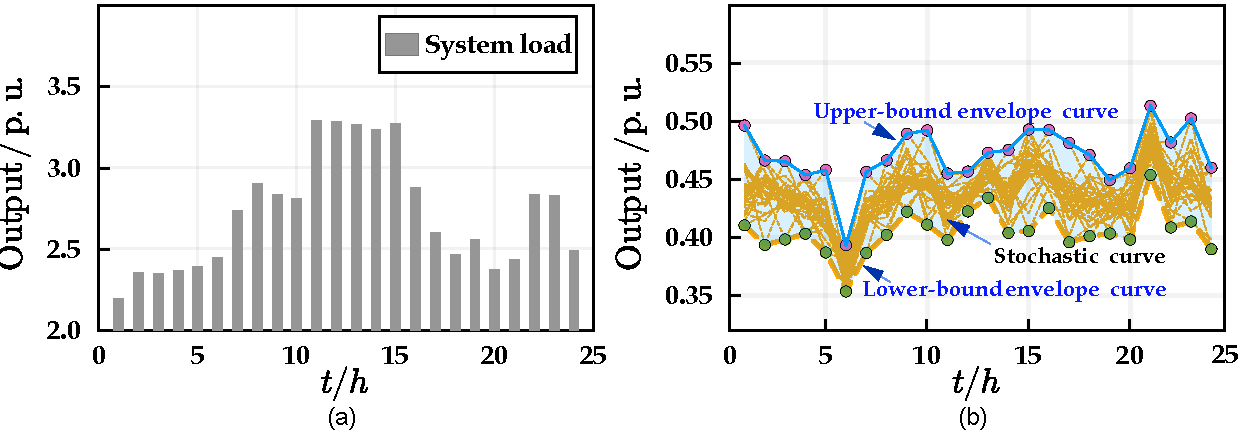
\includegraphics[width=1.0\linewidth]{fig8_LOADandWINDscurves}
	\caption{System load curve in (a) and stochastic wind power scenarios in (b) in the modified IEEE 6 bus test system.}
	\label{fig5}
	\vspace{-0.1cm}
\end{figure}
\begin{figure}[!t]\vspace{-0.35cm}
	\centering
	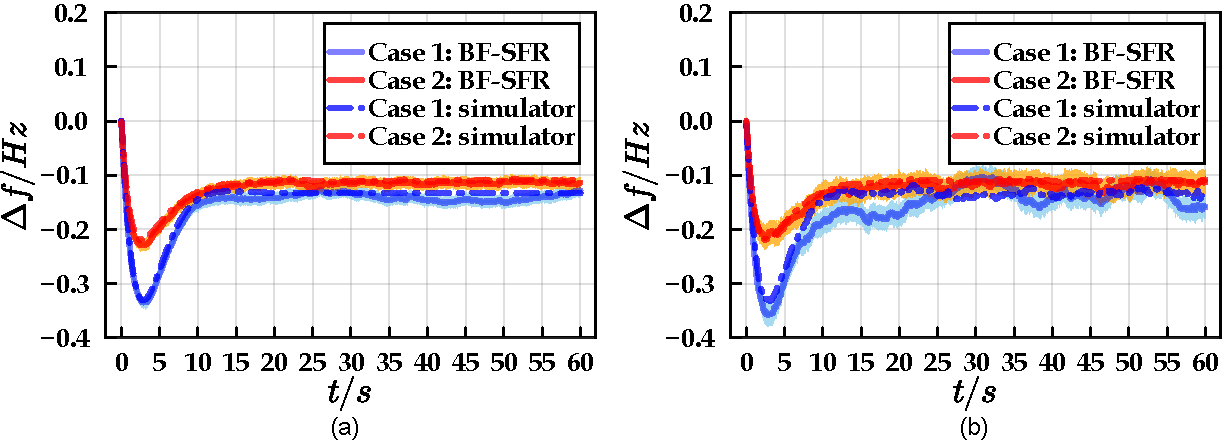
\includegraphics[width=1.0\linewidth]{fig5_new_SFRcurves}
	\caption{Frequency curves of BF-SFR/simulator with little residual setting in (a) and large residual condition in (b).}
	\label{fig6}
\end{figure}
\begin{figure}[!t]\vspace{-0.5cm}
	\centering
	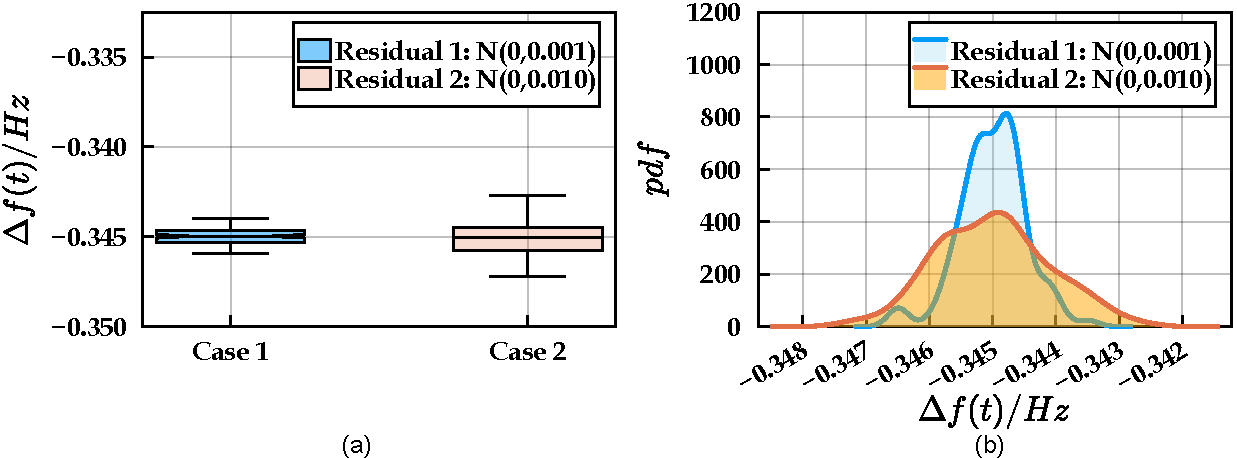
\includegraphics[width=1.0\linewidth]{fig6_SFRPDFinformations}
	\caption{Statistical $\nicefrac{1}{2}$ and $\nicefrac{1}{4}$ quantile level in (a) and posterior probabilistic density distribution in (b) of $\varDelta f(t)$ at time-to-nadir under different residual conditions.}
	\label{fig7}
\end{figure}
\begin{figure}[!t]\vspace{-0.15in}
	\centering
	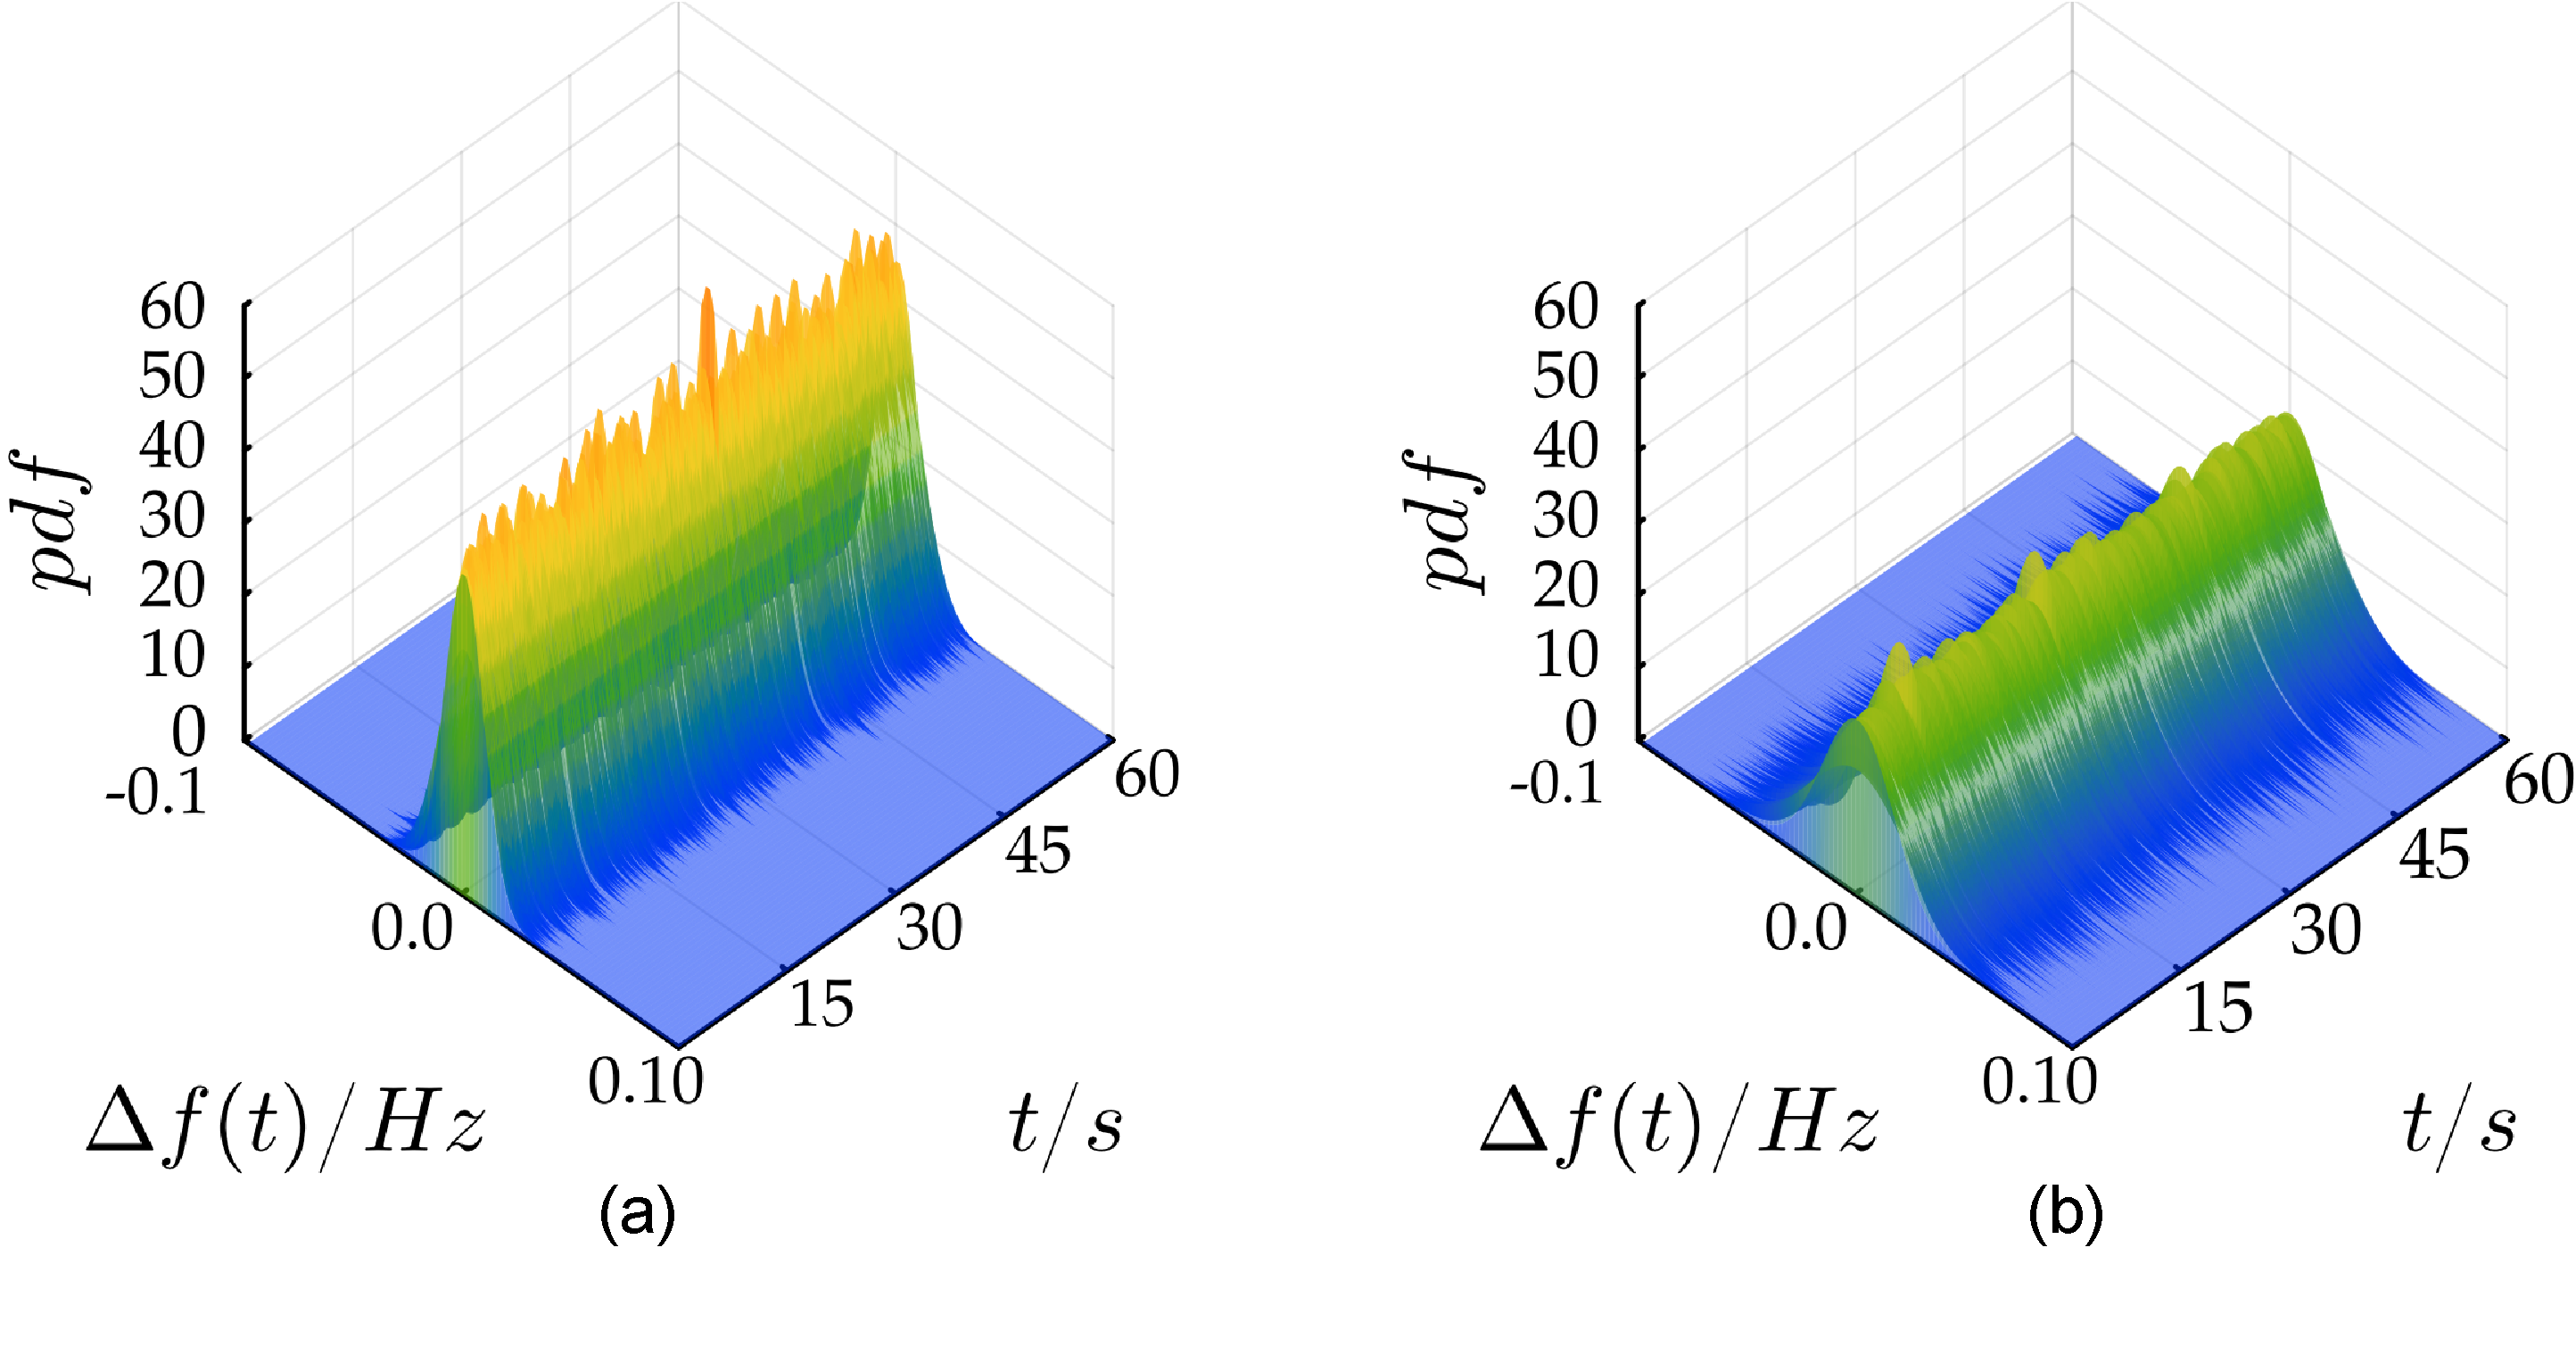
\includegraphics[width=0.9\linewidth, height = 1.25in]{fig7_surface.pdf}
	\caption{Union probabilistic density distribution of $\varDelta f(t):t\in[0s, 60s]$ under minor residual condition $N(0,0.001)$ in (a) and relatively large residual condition $N(0, 0.01)$ in (b).}
	\label{fig8}
\end{figure}

In Fig.~\ref{fig8}, the probabilistic density distribution of $\varDelta f(t)$ converges to a certain distribution at the end of the simulation time, it reflects that SFR in this case has a stationary probabilistic distribution. Especially, the distribution of $\varDelta f(t)$ at the minor residual condition is sharper than its counterpart at the relatively large residual condition, leading to reduced uncertain risks. Hence, the security of frequency dynamic can be well maintained if limited UV factors are incorporated. On the contrary, if there are a great number of UV derivation from converters introducing into the grid, the possible value of  $\varDelta f(t)$ would become broader, it leads to a difficult prediction and re-dispatching issue. Therefore, the binding of SFR at a significant UV residual condition is essential by defining the $\nicefrac{1}{2}$ quartile and $\nicefrac{1}{4}$ quartile filtered from sampled frequency dynamic $filters$ (see Fig. \ref{fig7}(b)) through the proposed BF-SFR method.

\textit{A.2.  $TUC \,\, v.s. \,\, FDUC \,\, v.s. \,\, CCFCUC(the \,\,proposed)$}

To check the performance of introducing frequency dynamic requirements via BF-SFR into UC problems, TUC, \cite{7822944}, and recent previous frequency-dynamic UC (FDUC) model, \cite{zhang2020modeling}, are applied as benchmarks and sequentially compared with the proposed CCFDUC model (see \eqref{20-a} –  \eqref{21-n}). The differences between FDUC and CCFDUC lie in the construction of frequency nadir constraints. In the context of boundary conditions representing frequency dynamic requirements, the limit of RoCoF and nadir are, respectively, $1.0 Hz/s$ and $0.5 Hz$. The residual condition describing UV derivation during frequency dynamic processes is $\langle\varpi,\sigma\rangle\in N(0,0.001)$. Accordingly, Fig. 10 compares the calculated scheduled costs and commitment results produced by TUC, FDUC and CCFDUC.

\begin{table}[!t]\vspace{-0.35cm}
	\caption{Scheduled cost including units' shut-on cost, shut-down cost and fuel cost produced by TUC/FDUC/CCFDUC.}\label{table 4}
	\resizebox{0.49\textwidth}{0.3in}{\begin{tabular}{lrrrr}
			\hline
			Models & shut-up cost           & shut-down cost        & fuel cost             & total cost              \\
			\hline
			TUC    & $9.10\times 10^3 \$  $ & $3.50\times 10^3 \$ $ & $4.04\times 10^5\$ $  & $ 4.10\times 10^5 \$ $  \\
			FDUC   & $9.10 \times 10^3 \$ $ & —                     & $4.81\times 10^5 \$ $ & $ 4.90\times 10^5 \$ $  \\
			CCFDUC & $9.10 \times 10^3 \$ $ & —                     & $4.82\times 10^4 \$ $ & $ 4.91 \times 10^5 \$ $ \\
			\hline
		\end{tabular}}
\end{table}

In Table~\ref{table 3}, both schedule costs solved by FDUC\,/\,CCFDUC are close, it demonstrates the feasibility of integrating SFR via BF-SFR into UC. In comparison with the latter two frequency-dynamic UC models, all units' fuel cost through TUC is minor than that through FCUC and CCFDUC, while units' shut-on/shut-down costs using TUC are higher than its counterpart. It reflects that more conventional generators run at a bit uneconomical level in FDUC/CCFDUC over the entire dispatching horizons but only similar activated generators exist in TUC during limited peak-load periods for the sake of active power balance restriction. Note that FDUC/CCFDUC consider the frequency supporting benefit from wind farms and BESS, these grid-connected devices must preserve a certain frequency containment reserve for keeping adequate frequency regulation capacities. In this perspective, these grid-connected generators other than conventional generators through FDUC/CCFDUC run at a lack of economic point compared with the one via TUC. Therefore, activated conventional generators through FDUC/CCFDUC must produce more output for keeping active power balance. The comparison of accumulated output of conventional generators through TUC ($24.976 MW$), FDUC ($26.404 MW$ in Fig.~\ref{fig10}(a)) and CCFDUC ($26.402 MW$ in Fig.~\ref{fig10}(b)) demonstrated this explanation.

\begin{figure}[!t]\vspace{-0.25cm}
	\centering
	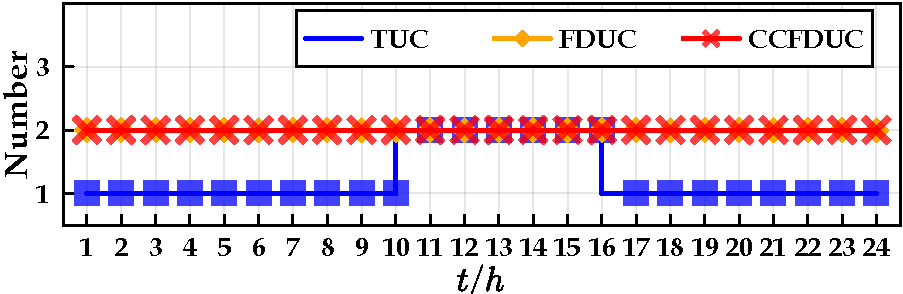
\includegraphics[width=0.8\linewidth,height=0.85in]{fig9_OnlineUnitRes}
	\caption{Cumulative numbers of activated conventional generators through TUC/FDUC/CCFDUC in the modified IEEE 6 bus test system.}
	\label{fig9}
\end{figure}

Furthermore, the number of activated conventional generators in Fig. \ref{fig9} through TUC is broadly minor than that through FDUC/CCFDUC expect for limited peak-load periods. This issue can be more pronounced at 1h$-$9h and 17h$-$24h. During these period internals, only G1 is activated through TUC but G1 and G2 keep online through FDUC/CCFDUC. It is because that the scheduled generators produced by frequency-dynamic UC schemes must dispatch more conventional generators to keep online in order to maintain an appropriate inertia level, but this issue is implicitly ignored in the TUC. Therefore, a conclusion can be drawn that the impact of incorporating SFR problems into UC would bring more generators to keep online to maintain a suitable inertia degree and frequency supporting capacity, resulting in safer frequency dynamic response against mismatch power disturbance.

\begin{figure}[!t]\vspace{-0.2in}
	\centering
	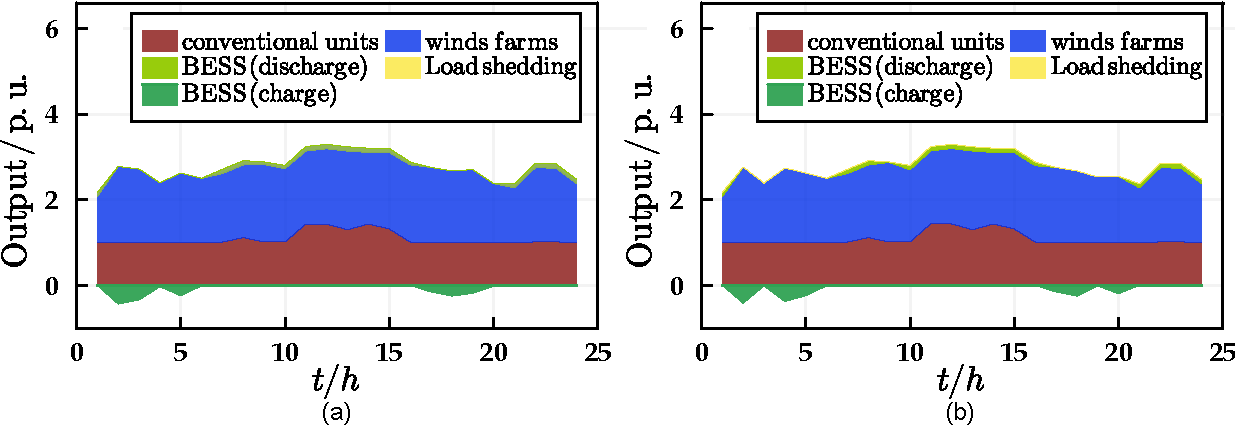
\includegraphics[width=1.0\linewidth]{fig10_powerbalance2and3}
	\caption{Active power balance curves of calculated scheduled commitments produced by TUC/FDUC/CCFDUC in the modified IEEE 6 bus test system.}
	\label{fig10}
\end{figure}

To compare the effectiveness of introducing SFR via BF-SFR into UC studies, Fig.~\ref{fig11} statistics chronological curves of RoCoF and frequency nadir regarding scheduled commitments produced by TUC/FDUC/CCFDUC. It can be found that the scheduled results through FDUC/CCFDUC satisfy predefined frequency dynamic thresholds, but TUC does not. As a result, the necessity of introducing SFR into UC issues can be well demonstrated.

\begin{figure}[!t]\vspace{-0.2in}
	\centering
	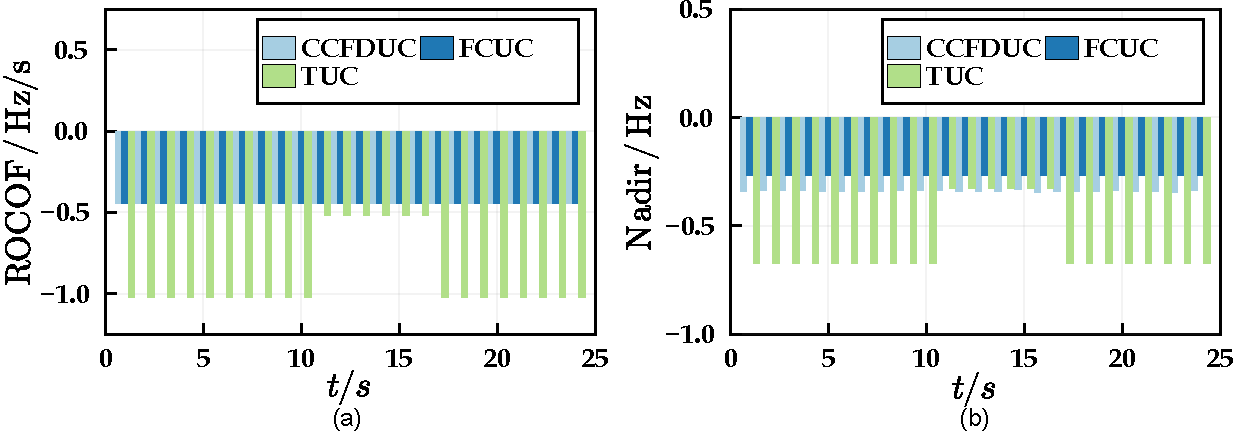
\includegraphics[width=1.0\linewidth]{fig11_RoCOFandnadirdistributionINFO}
	\caption{The distribution of RoCoF in (a) and nadir in (b) corresponding to scheduled commitments through TUC/FDUC/CCFDUC in the modified IEEE 6 bus test system.}
	\label{fig11}
\end{figure}

Nevertheless, the values of RoCoF/nadir with similar commitment results in Fig.~\ref{fig11} solved by TUC and FDUC/CCFDUC still has a slight difference. This phenomenon can be found and highlighted at 11h$-$16h in Fig. \ref{fig11}. At these periods, both calculated commitment results through TUC/FDUC/CCFDUC are similar, i.e., G1/G2 is on and G3 is off. In spite of this, there still exist several improvements of RoCoF and frequency nadir in the scheduled results produced by FDUC/CCFDUC. It is because that wind farms and BESS are took into account to participate into frequency supporting within FDUC/CCFDUC but TUC does not. Since the maximum of RoCoF is inversely proportional to the system inertia according to eq.\eqref{eqn:10}, thereby, the integrating of wind farm with VI control can increase the system inertia and reduce RoCoF, and the benefit of droop-controlled wind farm and BESS results in an increase in available frequency regulation capacity, facilitating smoother frequency response and adequate frequency reserve inspired by \cref{eqn:11,eqn:14,eqn:19}. The specific frequency curve of scheduled commitments via TUC/FDUC/CCFDUC at $t=10$h in Fig. \ref{fig13} verified this explanation. It can be found in Fig. \ref{fig13} that the frequency nadir using FDUC/CCFDUC is smaller than that through TUC, leading to smoother frequency response curve and adequate frequency reserve.
% In combination with the above discussion, the significance of wind farms and BESS participating in SFR in UC problems can be observed.
\begin{figure}[!t]\vspace{-0.25in}
	\centering
	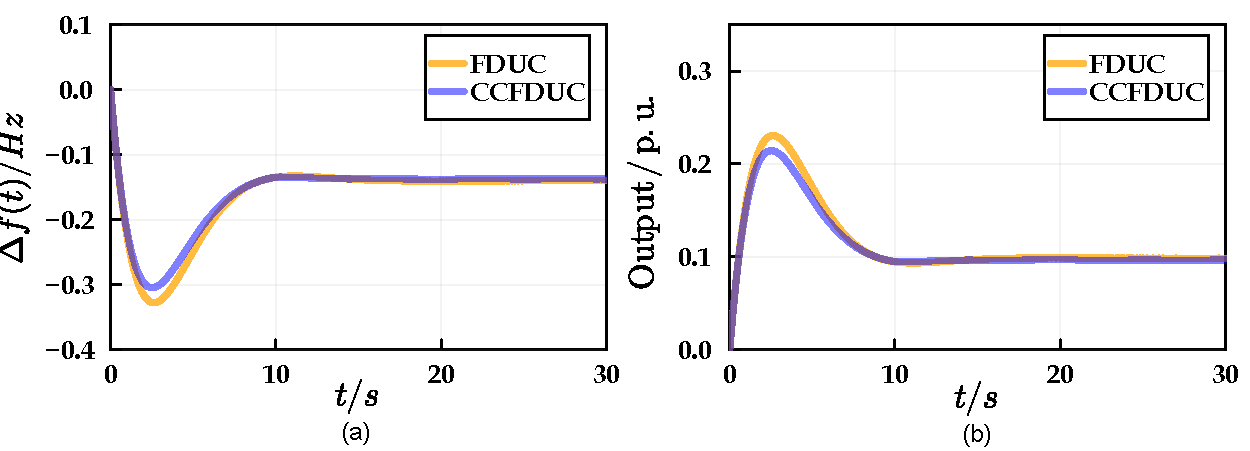
\includegraphics[width=1.0\linewidth]{fig13_SFRcurveandadditionaPower}
	\caption{Frequency dynamic curves in (a) and additional output in (b) through TUC/FDUC/CCFDUC in the modified IEEE 6 bus test system.}
	\label{fig13}
\end{figure}

\begin{figure}[!t]\vspace{-0.125in}
	\centering
	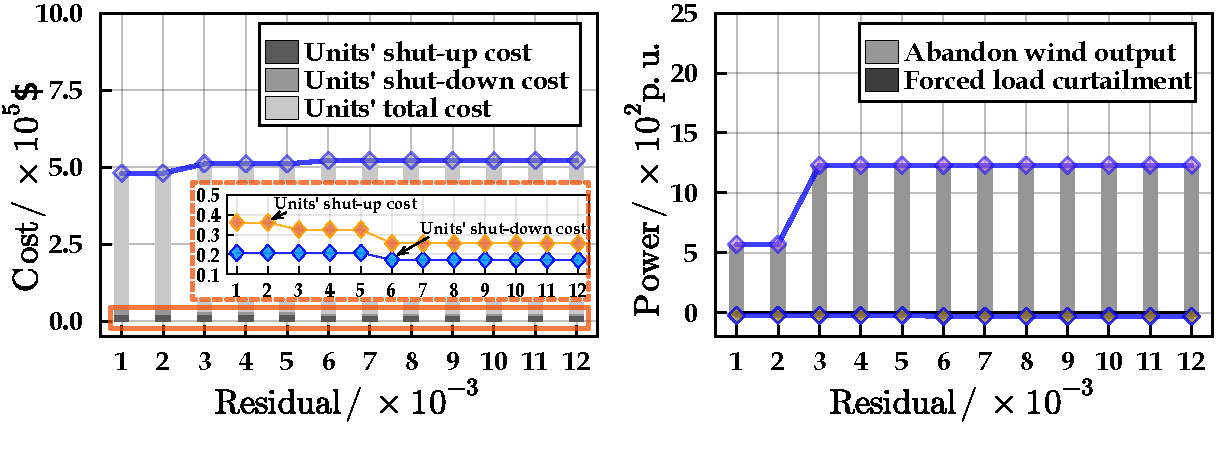
\includegraphics[width=\linewidth]{fig12_cost_and_wastepower}
	\caption{Change of scheduled cost and abandoned power through CCFDUC with different residual settings.}
	\label{fig12}
\end{figure}

Next, Fig.~\ref{fig12} explores the evolution of scheduling results via CCFDUC with various residual settings. The scheduling cost will rise with the increase of external residual influences; in the meantime, the risk of abandoned wind output and forced-load-curtailment for preventing power-balance violation would also increase. As the residual changes within a relatively low internal between $1\times 10^{-3}$ and $2\times 10^{-3}$, the scheduling cost through CCFDUC increases slowly, it indicates that the minor residual has a negligible effect on the final scheduling result. However, when the residual changes from $2\times 10^{-3}$ to $3\times 10^{-3}$, the scheduling results have a relatively obvious increase. This is mainly because some inactivated units in previous minor residual settings are required to be shut up in such condition. And, when the residual continuously increases from $3\times 10^{-3}$ to $10\times 10^{-3}$, due to the fact that more units keep active and the system inertia has maintained at a relatively high degree, hence, the scheduling cost and power abandonment growth are maintained at a relatively flat curve. From this perspective, the necessity and significance of introducing UV  into UC studies is well clarified.
%\begin{figure}[!t]
%\centering
%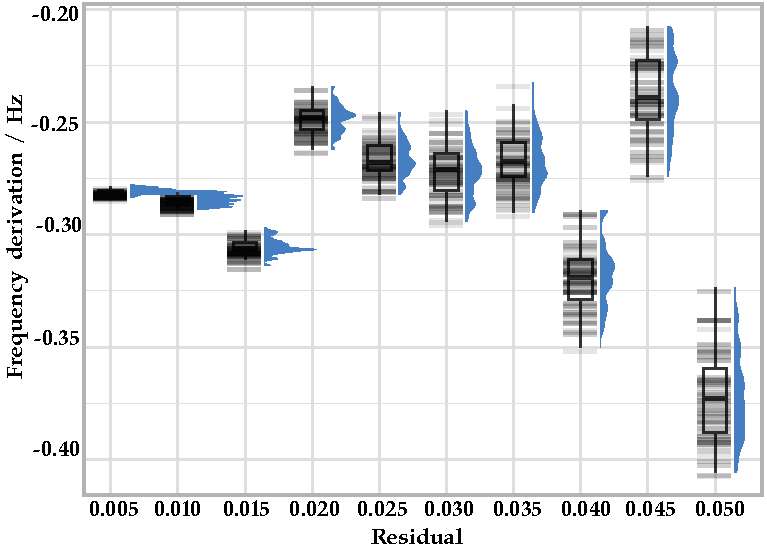
\includegraphics[width=0.9\linewidth]{fig13_CloudRainVis}
%\caption{The unified frequency dynamic response of electrical power systems against occurred power disturbance}
%\label{fig12}
%\end{figure}

\vspace{-0.2in}
\subsection{Modified IEEE 118 test system}
\vspace{-0.08in}

The system contains \!$54$ conventional units, \!$186$ lines and \!$91$ loads. The cumulative installed capacity of conventional generators amounts to $7,220$MW, while the peak-load reaches $5,516.08$MW.
In addition, the system encompasses $3$ wind farms $\langle \textrm{G}55,\textrm{G}56,\textrm{G}57\rangle$, located on buses $\langle 24,25,26\rangle$, respectively. Each wind farm has a installed capacity of $500$MW. The criteria of RoCoF and nadir are $2.0$Hz/s and $0.5$Hz. More boundaries about all units' physical operation parameters and frequency parameters can be found in Ref.~\cite{demetriou2015dynamic}. an increase of load (approximately $10\%$ of peak load) is chosen to define a representative power disturbance. Table \ref{table 4} presents the dispatching costs through TUC/FDUC/CCFDUC. Meanwhile, Fig. \ref{fig12} statistics the number of activated generators over the dispatching horizon. Figure 19 illustrates the change of RoCoF and nadir in relation to various obtained scheduling commitments through TUC/FDUC/CCFDUC.

\begin{table}[!t]\vspace{-0.35cm}
	\caption{Scheduled cost including units' shut-on cost, shut-down cost and fuel cost produced by TUC/FDUC/CCFDUC.}\label{table 3}
	\resizebox{0.49\textwidth}{0.3in}{\begin{tabular}{lrrrr}
			\hline
			Models & shut-up cost          & shut-down cost       & fuel cost             & total cost             \\
			\hline
			TUC    & $1.54\times 10^4 \$ $ & $0.31\times 10^4 \$$ & $1.62\times 10^6\$  $ & $1.64 \times 10^6 \$ $ \\
			FDUC   & $4.18\times 10^4 \$ $ & $2.71\times 10^4 \$$ & $1.73\times 10^6 \$ $ & $1.81 \times 10^6 \$ $ \\
			CCFDUC & $3.49\times 10^4 \$ $ & $1.67\times 10^4 \$$ & $1.81\times 10^6 \$ $ & $1.86 \times 10^6 \$ $ \\
			\hline
		\end{tabular}}
\end{table}

%Therefore, the percentage of wind farms for the peak-load is $20.79\%$.
\begin{figure}[!t]\vspace{-0.2in}
	\centering
	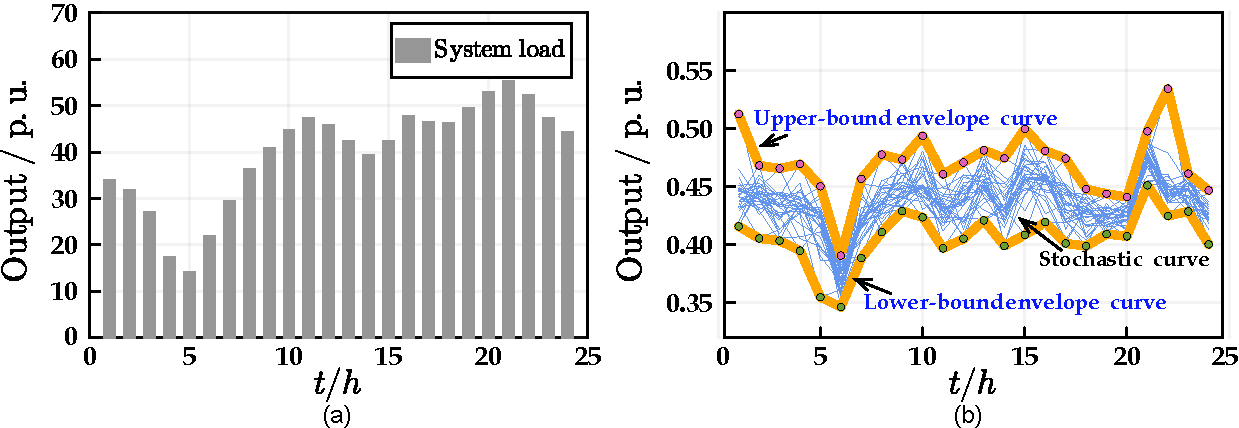
\includegraphics[width=1.0\linewidth]{fig14_bigcase_LOADandWINDscurves}
	\caption{Load curve in (a) and stochastic wind power scenarios in (b) in the modified IEEE 118 bus test system.}
	\label{fig12}
\end{figure}

\begin{figure}[!t]\vspace{-0.225in}
	\centering
	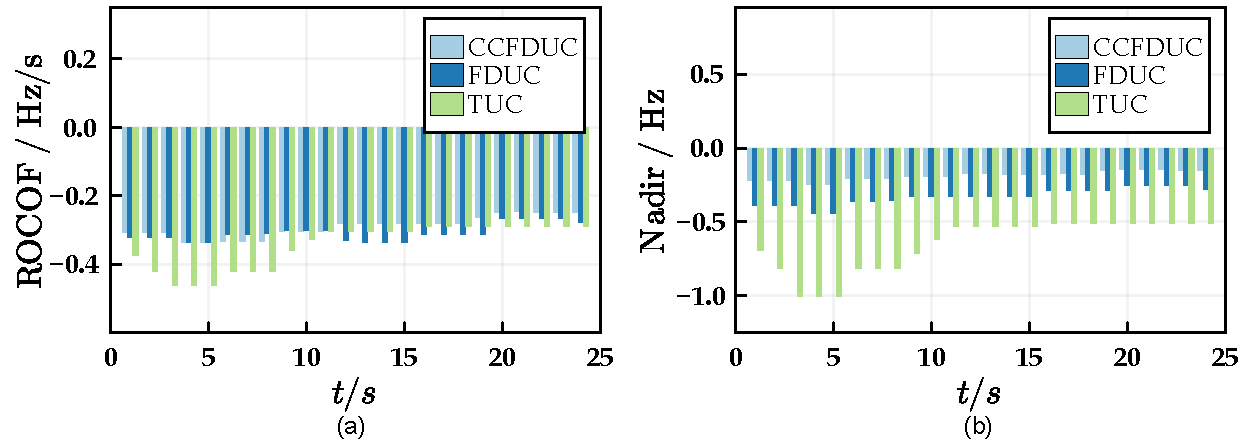
\includegraphics[width=1.0\linewidth]{fig15_bigcase_RoCOFandnadirdistributionINFO}
	\caption{The distribution of RoCoF in (a) and nadir in (b) corresponding to  scheduled commitments through TUC/FDUC/CCFDUC in the modified IEEE 118 bus test system.}
	\label{fig12}
\end{figure}

\begin{figure}[!t]\vspace{-0.125in}
	\centering
	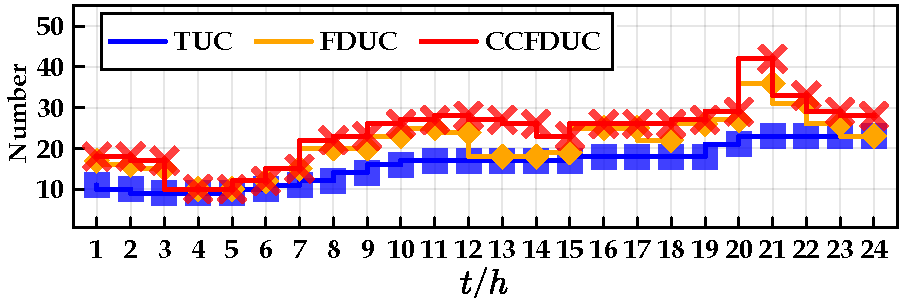
\includegraphics[width=0.8\linewidth, height=0.85in]{fig16_bigcase_OnlineUnitRes}
	\caption{Cumulative numbers of activated conventional generators through TUC/FDUC/CCFDUC in the modified IEEE 118 bus test system.}
	\label{fig12}
\end{figure}

% The calculated costs solved by TUC/FDUC/CCFDUC are, respectively, $1.642 ×10^6$ and $1.655 ×10^6$.
In table \ref{table 4}, the scheduled costs and activated units' number through FDUC/CCFDUC exhibit a bit greater value compared to those through TUC. The major distinction for this difference lies in an reconsideration of frequency dynamic requirements. Such units with adequate frequency regulation capabilities are prioritized in FDUC/CCFDUC, and this selection of active generators utilizing this logicism is particularly evident during low-load periods (see scheduling periods $3h\!-\!6h$ in Fig.~\ref{fig12}). It can be observed in Fig. \ref{fig12} that the number of activated generators  through TUC is lower compared to those activated through FDUC/CCFDUC. It is because that the system necessitates a restricted number of conventional generators for maintaining power balance. Nevertheless, these activated generators behind TUC may not provide an adequate level of the system inertia, resulting in a limited capability for these units to keep frequency dynamic security. Therefore, supplementary generators are compelled to remain operational with a reduced output so as to sustain the required amount of the system inertia.

The number of activated generators using FDUC and CCFDUC exhibits similarity, hence reinforcing the validity of the suggested model. Nevertheless, there are still minor disparities in the scheduled results employed by these two models under restricted dispatching intervals. For instance, at a specific time of $21$h, the number of conventional generators determined by FDUC is $36$, but the number determined using CCFDUC is $40$. The discrepancy between FDUC/CCFDUC can be attributed to the altered formulation of frequency restrictions that pertain to frequency dynamic security. The frequency constraints in FDUC stem from a analytical SFR approach, \cite{paturet2020stochastic,anderson1990low, shi2018analytical}, with an implicitly free UV assumption. In contrast, the frequency limits in CCFDUC are based on the BF-SFR that incorporates specific UV assumptions. Given the consideration of both the advantages of additional frequency control through converters and the associated fluctuations that may lead to UV residuals, CCFDUC tends to strike a balance, and this balance involves maximizing the incorporation of converters to enhance system frequency security while mitigating the adverse impact of UV issues. Noted that the nadir exhibited by CCFDUC is superior to that of FDUC. This indicates a higher level of robustness in terms of scheduling obligations.

% In particular, the number of conventional generators soluted by TUC/FCUC at period $5$h are $9$ and $11$, respectively. However, units $21, 29$ and $51$ are additionally scheduled to participate in frequency support through FCUC, while the generator $26$ is inactivated. Since these generators almost have significant inertia and droop coefficient compared with the rescheduled generator $26$ within TUC, hence, a conclusion can be made that, FCUC trends to recall generators with better frequency control performance for providing inertia supporting if the frequency dynamic requirement is incorporated. The results of conventional states through TUC/FCUC at period 5 in Fig. 14 have explained this issue.

% It can be found on Fig. 20 that both RoCoF and nadir distributions of scheduled results over the entire operation periods via en-hance FCUC perfectly meet predefined frequency dynamic requirements, but TUC does not. Especially during these periods from 1h to 7h, both changes of RoCoF and frequency nadir through TUC are almost higher than the threshold of frequency dynamic requirement, which may happen frequency instability issues. From this point, it again declares that the rescheduled result of FCUC keeps a good frequency dynamic response with frequency constraints into reconsideration.

% Furthermore, Fig. 21 compares the frequency dynamic of scheduled commitment produced by generators at period 6h through TUC and FCUC. It can be observed that the frequency nadir of scheduled commitment through FCUC is smaller than that by utilizing TUC, lead-ing to safer frequency dynamic response. In combination with this discussion, the effectiveness of FCUC concerning big-size power systems can be well demonstrated.
\vspace{-0.125in}
\section{Conclusion}
\vspace{-0.05in}

This paper presents a novel well-designed BF-SFR method for encoding frequency dynamic requirements in CCFDUC. The suggested model allows for a flexible consideration of sophisticated frequency control schemes and stochastic residuals representing UV issues. Furthermore, the convex reformulation of the chance-constraint nadir constraints derived from BF-SFR is discussed. Two cases are then carried out to check the validness and scalability of BF-SFR and FDUC methodologies.

Three findings indicate that:
$i)$	The trajectory of frequency derivation solved by BF-SFR is consistent with the simulated curve, and the probabilistic distribution of frequency derivation under different residual settings can be well visualized through BF-SFR.
$ii)$	Introducing frequency dynamic requirement in UC problems may increase the scheduled cost and the number of grid-connected generators, nevertheless, the resulting scheduling result from FDUC/CCFDUC is beneficial in terms of ensuring system frequency security.
$iii)$	CCFDUC has better performance in balancing the participation of converters in frequency support and avoiding excessive UV perturbations.


\bibliographystyle{ieeetran}
\vspace{-0.1in}
\noindent{\fontfamily{stix}\selectfont
	\fontsize{9}{9.5}\selectfont
	\bibliography{reference}}
\end{document}


